\documentclass[12pt]{book}
\usepackage{imakeidx}
\usepackage{graphicx}
\usepackage{amssymb}
\usepackage[most]{tcolorbox}
\tcbset{noparskip}
\usepackage{multicol}
\usepackage{ifthen}
\usepackage{color}
\usepackage{setspace}
\usepackage{amsthm, amsmath}
\usepackage{pdfpages}
\usepackage{tikz}
\usepackage{url}
\usetikzlibrary{arrows}
\usepackage{extramarks}
\usepackage{letltxmacro} %
\usepackage{amsfonts}
\usepackage{tikz}
\usepackage[plain]{algorithm}
\usepackage{algpseudocode}
\usepackage{chngcntr}
\usepackage{listings}
\usepackage{enumitem}
\usepackage{amsmath, amssymb, amsthm, multicol, setspace}
\usepackage{graphicx}
\usepackage{xcolor}
\usepackage{tikz}
\usepackage{mathrsfs}
\usepackage{pdfpages}
\usepackage{gensymb}
\usepackage{scrextend}
\usepackage{array}
\usepackage{pst-solides3d}
\usepackage[OT1]{fontenc}
\usepackage[colorlinks=true, allcolors=black]{hyperref}
\usepackage[capitalize,nameinlink]{cleveref}
\usetikzlibrary{arrows}
\usetikzlibrary{calc}
\usetikzlibrary{automata,positioning}
\usetikzlibrary{shapes.geometric}
\usepackage{geometry}
\geometry{papersize={8.5in,11in}, hmargin={1.25in, 1.25in}, bindingoffset=0.25in, height=8.5in, top=1in, headheight=15pt, twoside, ignoreheadfoot}

% No section numbers:
\setcounter{secnumdepth}{0}

\doublespacing

\newtheorem{theorem}{Theorem}

\theoremstyle{definition}
\newtheorem{definition}{Definition}
\newtheorem{example}{Example}

\def\Z{\mathbb{Z}}

\usepackage[utf8]{inputenc}
\usepackage[T1]{fontenc}
\usepackage{newpxtext}
\usepackage[vvarbb,cmintegrals,cmbraces,bigdelims]{newpxmath}
\usepackage[scr=rsfso]{mathalfa}% \mathscr is fancier than \mathcal
% \linespread{1.04}         % adds more leading (space between lines)
% quantifiers look strange, so change those back to normal:
	\DeclareSymbolFont{mysymbols}{OMS}{cmsy}{b}{n} %note we make the figures bold to better match newpx.  Replace the ``b'' with an ``m'' to undo this.
	%\SetSymbolFont{mysymbols}  {bold}{OMS}{cmsy}{b}{n}
	%\DeclareSymbolFont{myoperators}   {OT1}{cmr} {m}{n}
	%\SetSymbolFont{myoperators}{bold}{OT1}{cmr} {bx}{n}
	\DeclareMathSymbol{\forall}{\mathord}{mysymbols}{"38}
	\DeclareMathSymbol{\exists}{\mathord}{mysymbols}{"39}
	%\DeclareMathSymbol{\pm}{\mathbin}{mysymbols}{"06}
	%\DeclareMathSymbol{+}{\mathbin}{myoperators}{"2B}
	%\DeclareMathSymbol{-}{\mathbin}{mysymbols}{"00}
	%\DeclareMathSymbol{=}{\mathrel}{myoperators}{"3D}

%%%%%%%%%%%%%%%%%%%%%%%%%%%%%%%%%%%%%%%%%%
%%%%%%%  Headers and footers %%%%%%%%%%%%%
%%%%%%%%%%%%%%%%%%%%%%%%%%%%%%%%%%%%%%%%%%
\usepackage{fancyhdr}
\pagestyle{fancy}
\renewcommand{\chaptermark}[1]{\markboth{\thesection.\ #1}{}} %Removes word "chapter" from the \leftmark.


\fancyhead{} % clear header fields
\fancyhead[LE]{{\footnotesize \textsl{\thepage}}~~ \textsc{\scriptsize \nouppercase{\leftmark}}}
\fancyhead[RO]{\textsc{\scriptsize \nouppercase{\rightmark}} ~~ {\footnotesize \textsl{\thepage}}  }
\fancyfoot{}

%%%%%%%%%%%%%%%%%%%%%%%%%%%%%%%%%%%%%%%%%%
%%%%%%%    Chapter headings  %%%%%%%%%%%%%
%%%%%%%%%%%%%%%%%%%%%%%%%%%%%%%%%%%%%%%%%%

\usepackage{titlesec}


%%%%%%%% SUBSECTION  TITLE SPACING ISSUE-FIX %%%%%%%%%%%%%%%%%
\titlespacing{\subsection}{0pt}{\parskip}{-\parskip}
%%%%%%%%%% INDEX %%%%%%%%%%%%%%%
\makeindex[intoc,title= Primer Index]

%%%%% FIX FOR BUG IN TITLESEC %%%%%%%%%%%
\usepackage{etoolbox}

\makeatletter
\patchcmd{\ttlh@hang}{\parindent\z@}{\parindent\z@\leavevmode}{}{}
\patchcmd{\ttlh@hang}{\noindent}{}{}{}
\makeatother
%%%%% END FIX %%%%%%%%%%%%%%%%%%%%%%%%%%%%


% \titleformat{\chapter}[display]
% 	{\Large\filcenter}
% 	{\rule[4pt]{.3\textwidth}{2pt} \hspace{2ex} \large\textsc{\chaptertitlename} \thechapter \hspace{3ex} \rule[4pt]{0.3\textwidth}{2pt} }
% 	{1pc}
% 	{\titlerule\vspace{1ex}\huge\textsc}
% 	[\vspace{.75ex}\titlerule]
% \titlespacing*{\chapter}{0pt}{-2em}{2em}

\titleformat{\subsection}[block]
  {\normalfont\bfseries\filcenter}
  {\theparagraph}
  {}
  {\textsc}

\newcommand{\sectionbreak}{\clearpage\thispagestyle{plain}}
\titleformat{\section}[block]
  {\Large\bfseries\filcenter}
  {\theparagraph}
  {}
  {\textsc}
%%%%%%%%%  End chapter/sectio headings %%%%%%%%%%%%%%%%%

%%%%% odd enumeration command %%%%%
\newlist{oddenumerate}{enumerate}{1}
\setlist[oddenumerate]{start=0,label=\theoddenumeratei.}
\makeatletter
\renewcommand\theoddenumeratei{\@arabic{\numexpr2*\value{oddenumeratei}+1}}
\makeatother



%%%%New_tccolorbox_environments%%%%%%%%%%%%%%%%%%%%%%%%%%%%%%%%%%%%%%%%%%%%%%%%%%%%%%%%%%%%%%%

%%counters_for_tccolorbox_designs%%
\newcounter{tctheoremcounter}[section]
\newcounter{tcexamplecounter}[section]


%%%newtheoremdesign%%%%
\newtcbtheorem[use counter=tctheoremcounter]{tctheorem}{Theorem}{%
	lower separated=false,
	colback=white,
	colframe=black,fonttitle=\bfseries,
	colbacktitle=gray!20,
	coltitle=black,
	top = .5em,
	before skip=2ex,
	after skip=2ex,
	breakable,
	enhanced,
	boxed title style={boxrule=0pt,colframe=white,},
}{tctheorem}


%%%newexampledesign%%%%
\newtcbtheorem[use counter=tcexamplecounter]{tcexample}{Example}{%
	lower separated=false,
	colback=white,
	colframe=black,fonttitle=\bfseries,
	colbacktitle=black,
	coltitle=white,
	top = 1.25em,
	before skip=2ex,
	after skip=2ex,
	breakable,
	enhanced,
	attach boxed title to top left={yshift=-0.11in,xshift=0.15in},
	boxed title style={boxrule=0pt,colframe=white,},
}{example}



%%%%newproofdesign %%%%%
\newtcolorbox{newproof}[1][]{%
	enhanced,
	breakable,
	fonttitle=\bfseries,
	title=Proof:,
	coltitle=black,
	frame hidden,
	colback=white,
	before skip=2ex,
	after skip=2ex,
	attach title to upper=\quad,
	overlay unbroken={%
		\draw[thick,black,double] ([yshift=-7pt]interior.north west)--(interior.south west)--(interior.south east);
	},
	overlay first={
		\draw[thick,black,double] ([yshift=-7pt]interior.north west)--(interior.south west);
	},
	overlay middle={
		\draw[thick,black,double] ([yshift=-7pt]interior.north west)--(interior.south west);
	},
	overlay last={
		\draw[thick,black,double] ([yshift=-7pt]interior.north west)--(interior.south west)--(interior.south east);
	},
	#1, 
}

%%%%%%%%%%%%%%%%%%%%%%%%%%%%%%%%%%%%%%%%%%%%%%%%%%%%%%%%%%%%%%%%%%%%%%%%%%%%%%%%%%%%%%%%%%%%%%
\providecommand\phantomsection{}

%%%%%%%%%%%%%%%%%%%%%%%%%%%%


\begin{document}

\pagestyle{plain}
\pagenumbering{roman}




\thispagestyle{empty}


%~
%\tikz[remember picture, overlay] \node  at (current page.center){\includegraphics[width=\paperwidth,height=\paperheight]{images/titlebg}};


~
\vskip 1.75in

\begin{center}


\resizebox{.9\linewidth}{!}{\scshape Some Abstract Algebra}


\vskip 3em

% \tikz[scale=1]{
% \draw (0,0) rectangle (2,2);
% \draw (-0.2, -0.2) rectangle (2.2, 2.2);
% \draw (-0.4, -0.4) rectangle (2.4, 2.4);
% \draw (-0.6, -0.6) rectangle (2.6, 2.6);
% }

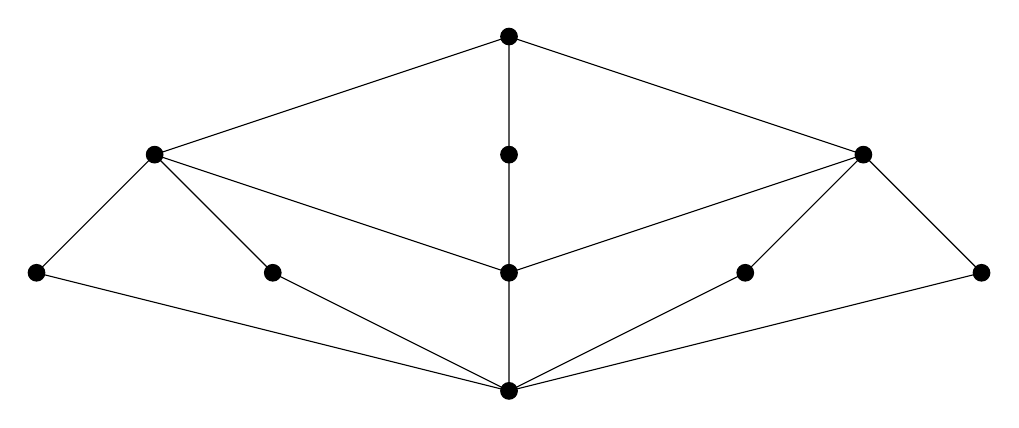
\begin{tikzpicture}[scale=1.5]
	\coordinate (h9) at (0,0);
	\coordinate (h8) at (4,1);
	\coordinate (h7) at (2,1);
	\coordinate (h6) at (0,1);
	\coordinate (h5) at (-2,1);
	\coordinate (h4) at (-4,1);
	\coordinate (h3) at (3,2);
	\coordinate (h2) at (0,2);
	\coordinate (h1) at (-3,2);
	\coordinate (h0) at (0,3);

	\draw[color=black] (h0) -- (h1) -- (h4) -- (h9) -- (h8) -- (h3) -- (h0) -- (h2) -- (h6) -- (h9) -- (h5) -- (h1) -- (h6) -- (h3) -- (h7) -- (h9);
	\foreach \i in {0,...,9}{
	\draw[fill=black, color=black] (h\i) circle (2pt);
	}
\end{tikzpicture}

\vskip 2em

\resizebox{.75\linewidth}{!}{\scshape A Primer and Interactive Workbook}



\vskip 1.5in

\resizebox{.75\linewidth}{!}{\scshape Richard Grassl \quad - \quad Tabitha Mingus}

\vskip .5in

% \resizebox{.2\linewidth}{!}{\scshape 2018}

\end{center}


%\includepdf[pages=-,pagecommand={\thispagestyle{empty}}]{frontmatter/cover2}
%
%

\clearpage






%\addtocontents{toc}{\protect\thispagestyle{plain}}

\thispagestyle{empty}
\vskip 1em

\noindent Richard Grassl \\[-1.5ex] Emeritus Professor of Mathematical Sciences \\[-1.5ex] University of Northern Colorado \\[-1.5ex] Greeley, Co 80639 \\[-1.5ex] \url{richard.grassl@unco.edu}

\vskip 1em

\noindent Tabitha Mingus \\[-1.5ex] Associate Professor of Mathematics \\[-1.5ex] Western Michigan University \\[-1.5ex] Kalamazoo, MI 49008


\vfill
\vfill
\noindent\textcopyright ~ 2018 by Richard Grassl

\vskip 3em

\noindent
\includegraphics[scale=.5]{frontmatter/by-sa}\\
This work is licensed under the Creative Commons Attribution-ShareAlike 4.0 International License. To view a copy of this license, visit\\ \url{http://creativecommons.org/licenses/by-sa/4.0/}.

\vfill

\noindent Summer 2018 Edition
\vskip 1em
% \noindent ISBN-10: 1534970746\\
% \noindent ISBN-13: 978-1534970748

\vfill

\noindent A current electronic version can be found for free at\\ \url{http://www.openmathbooks.org/someabstract/}
\vskip 2em

% \noindent Cover image: \emph{Tiling with Fibonacci and Pascal}.
\noindent Prepared for publication by Oscar Levin for Open Math Books
\vskip 2em

\clearpage


\section*{Preface}

This book consists of two parts: one, a primer designed to provide an adequate introduction to the essentials of abstract algebra and to some related number theory, and two, a workbook designed to enable the reader to interactively engage with colleagues in exploring the fascinating world of abstract algebra.

We have taken a problem solving approach -- the primer alone contains over 130 problems. So be prepared for minimal text material to read, combined with worksheets that extend and enhance text topics. These worksheets are designed to encourage discovery of interesting relationships between algebraic structures, geometry, mappings, and proofs.

Very little, if any, background in abstract algebra is needed for a course based on this Primer and the workbook. This material has been used successfully for over a decade with in-service secondary teachers seeking licensure or an MA degree in teaching mathematics.

In this book we embrace the oft-quoted maxim - ``You learn mathematics by doing mathematics.'' Such an effort leads to better understanding and deeper learning.

Finally, a valuable by-product: A significant number of teachers who have studied this material have incorporated a variety of the worksheets into their secondary curriculum as they encounter topics like closure, binary operations and their properties, modular arithmetic, and the structure of the integers (yes, GCD and LCM show up), and the rational and real numbers.

% This book is rebound under an open source license and is available in electronic format for free at \url{http://www.openmathbooks.org/someabstract/}.

\begin{flushright}
  Richard Grassl\\
  April 2019
\end{flushright}


\cleardoublepage


 \thispagestyle{empty}
\begin{tikzpicture}[remember picture,overlay]
	\node[inner sep=0] at (current page.center){%
		\includegraphics[width=8in]{SAAnewtitlepage.pdf}};
	
\end{tikzpicture}
 

% \rule{0in}{1in}\\
% \rule{.75in}{0in}\begin{minipage}{5in}

% \end{minipage}
\clearpage
\setcounter{tocdepth}{1}
% \rule{0in}{2in}\\



% \begin{minipage}{4in}
\tableofcontents
% \end{minipage}
\cleardoublepage
\pagenumbering{arabic}

\pagestyle{fancy}

\section*{Introduction}
An abstract algebra consists of a set of objects (integers, real numbers, permutations, polynomials, matrices, $\dots$), various binary operations, along with some properties (closure, inverses, commutativity,$\dots$). Examples of abstract algebras include groups, rings, integral domains, and fields. Operations include rotations of regular geometrical figures, ordinary and modular addition and multiplication, addition and multiplication of matrices and of polynomials, composition of permutation cycles, direct products and others.

In one sense the core ideas of algebra are abstracted out and viewed from a much larger lens. For example, the problem of finding analogues of the quadratic formula, around the mid 1500’s, led to the study of the symmetric groups which shed light on the nonsolvability of the general quintic.

Applications are plentiful. Among the many fields of study making significant use of algebraic structures we include cryptography, genetics, mineralogy, the study of molecular structures in chemistry, elementary particle theory in physics, Latin squares in statistical experiments, and finally, architecture and art.

Important contributors over the past several centuries include Joseph Lagrange, Niels Abel, Arthur Cayley, Emmy Noether, Gauss, Galois, Sylow among many others.
\clearpage


\section{Binary Operations}
\stepcounter{section}
The concepts of being commutative and associative are usually introduced to students as they study the four basic arithmetic operations of addition, subtraction, multiplication and division of integers.  These four operations denoted by $+,\,-\,\times,\, \div$ are examples of binary operations.\\[.1in]

Let $S$ be any set.  A \underline{binary operation} \index{binary operation} on $S$ is  a function $f:S\times S\rightarrow S$.  Sometimes a binary operation is depicted using the \underline{infix} notation $(m,n)\mapsto m\,\square\, n$, rather than the \underline{prefix} notation $f(m,n)$.  The following are examples of binary operations on $\mathbb{N}=\{0,1,2,3,\dots\}$.\\
$$\begin{array}{|c|c|}
\hline
\underline{\text{OPERATION}}&\underline{\text{INFIX NOTATION}}\\
\hline
f(m,n)=m+n & m\,\square\, n=m+n\\
\hline
f(m,n)=mn & m\,\square\, n=mn\\
\hline
f(m,n)=\text{gcd}(m,n) & m\,\square\, n=\text{gcd}(m,n)\\
\hline
f(m,n)=5^m\cdot n & m\,\square\, n=5^m\cdot n\\
\hline
\end{array}$$
Additional binary operations that will be of importance include
\begin{equation*}\begin{split}
f(x,y)&= x\div y \text{ on }S=\mathbb{R} \text{ where } y\neq0\\
f(m,n)& = m-n \text{ on } S=\mathbb{Z}=\{0,\pm1,\pm2,\dots\}\\
f(m,n)&=m+n-mn \text{ on }S=\mathbb{Z}\\
f(m,n)&=m+n-1 \text{ on }S=\mathbb{Z}\\
f(A,B)&=A\cup B \text{ on } P(S) \text{ for }S=\{\text{a,b,c}\}\\
f(A,B)&=A\cap B \text{ on } P(S) \text{ for }S=\{\text{a,b,c}\}
\end{split}\end{equation*}
Here, $\cup$ denotes union and $\cap$ denotes intersection.  Also, $P(S)$, the power set for $S$, is the set of all subsets of $S$.  As an example, if $S$=\{a,b\},then $P(S)$ = \{ $\emptyset$, \{a\}, \{b\}, \{a,b\} \}.

\subsection{Properties of Binary Operations}

Binary operations on a set $X$ may or may not satisfy the following properties:\\
\underline{Commutativity:}\index{commutative} $x\,\square\, y =y\,\square\, x$ for all $x,y$ in $X$.\\
\underline{Associativity:}\index{associativity} $x\,\square\,(y\,\square\, z)=(x\,\square\, y)\,\square\, z$ for all $x,y,z$ in $X$.\\
\underline{Identity:}\index{identity} An element $e\in X$ such that $x\,\square\, e=e\,\square\, x = x$ for $x$ in $X$ is called an identity for the binary operation $\square$.\\
\underline{Inverses:}\index{inverse} If $e$ is an identity under $\square$, an inverse of an element $a$ in $X$ is an element $b$ in $X$ such that $a\,\square\, b=e=b\,\square\, a$.

For example, the operation $+$ on $\mathbb{Z}$ is associative since $a+(b+c)=(a+b)+c$ for all $a,b,c$ in $\mathbb{Z}$.  Since $a+b=b+a$, + is commutative.  The element 0 serves as an identity $e$ since $0+a=a+0=a$.  Each element $a\in \mathbb{Z}$ has an inverse, namely $-a$.

One important characterization or consequence of the notation $f:A\times A\rightarrow A$ is that the result $f(m,n)$, or $m\,\square\, n$, must be an element in $A$; i.e., $A$ must be \underline {closed}\index{closed, closure} under the binary operation $\square$.  So divisibility, denoted $\div$, is not a binary operation on $N=\{0,1,2,\dots\}$ since $m\div n = \frac m n$ is not necessarily an integer.  But $\div$ is a binary operation on the set $\mathbb{R}^+$ of positive real numbers.  Notice that since $2\div3\neq3\div2$, $\div$ is not commutative.
\newpage
\begin{tcexample}{}{} 
Consider the binary operation $m\,\square\, n=3^m\cdot n$ on $\mathbb{N}=\{0,1,2,\dots\}$; show that $\square$ is \underline{not} associative.  The following single example accomplishes this:
$$1\,\square\,(0\,\square\, 1) = 1\,\square\, 1 = 3\text{ but }(1\,\square\, 0)\,\square\, 1 = 0\,\square\, 1 = 1$$
Does $\square$ have an identity?  it might be natural to try 0 or 1.  Since $0\,\square\, n = n$ but $n\,\square\, 0=0$, 0 is not an identity.  Since $1\,\square\, n = 3n$, 1 is not an identity.  No other element in $n$ works either;  without an identity, there are no inverses.
\end{tcexample}
\addtolength{\partopsep}{-.5in}
\begin{tcexample}{}{}
Union, $\cup\,$, is a binary operation on $P(S)$ where $S$=\{a,b,c\}.  Since $A\cup(B\cup C)=(A\cup B)\cup C$, $\cup$ is associative.   Since $\emptyset \cup A=A=A\cup\emptyset$ for all $A\in P(S)$, the empty set $\emptyset$ serves as an identity.
\end{tcexample}

When the set $A$ is finite, a binary operation $\square$ can be given by a matrix table where the element $x\,\square\, y$ is found at the intersection of row $x$ and column $y$.
\clearpage
\begin{tcexample}{}{}
Let $A=\{1,3,7,9\}$ and let $x\,\square\, y$ be the digit in the units position upon ordinary multiplication of $x$ and $y$.  This is sometimes written as $x\,\square\, y \equiv xy(\text{mod }10)$.  The matrix table is
$$\begin{array}{c|cccc}
\,\square\, & 1 & 3 & 7 & 9\\
\hline
1 & 1 & 3 & 7& 9\\
3 & 3 & 9 & 1& 7\\
7 & 7 & 1 & 9 & 3\\
9 & 9 & 7 & 3 & 1
\end{array}$$
This binary operation $\,\square\,:A\times A\rightarrow A$ is associative (you need to check $4\cdot4\cdot4=64$ cases), is commutative (from the symmetry of the table), has identity 1, and each element has an inverse as shown in the following table:
$$\begin{array}{c|cccc}
x & 1 & 3 & 7 & 9\\
\hline
\text{inverse of }x & 1 & 7 & 3 & 9
\end{array}$$%
\end{tcexample} 

\begin{tcexample}{}{}
	The binary operation $\circ$ on $A$=\{e, a, b\} given by the table below is associative, commutative and has e as an identity.  In the exercises you are asked to find inverses.\\
	\begin{minipage}{2in}
		$$\begin{array}{c|ccc}
		\,\circ\, & \text{e} &\text{a} & \text{b}\\
		\hline
		\text{e} & \text{e} & \text{a} & \text{b}\\
		\text{a} & \text{a} & \text{b} & \text{e}\\
		\text{b} & \text{b} & \text{e} & \text{a}
		\end{array}$$
	\end{minipage}

\end{tcexample}

\begin{tcexample}{}{}
Let $A=\{1,2,5,10\}$ and $m\,\square\, n = \text{gcd}(m,n)$, the greatest common divisor of $m$ and $n$.  The matrix table for $\square$ is given.  With some effort, you can show that $\square$ is associative.The table's symmetry verifies that the operation $\square$ is commutative.  In the exercises, you are asked to determine an identity and to see if there are inverses.
\begin{minipage}{3.5in}
	$$\begin{array}{c|cccc}
	\,\square\, & 1 & 2 & 5& 10\\
	\hline
	1 & 1 & 1 & 1 &1\\
	2 & 1 & 2 & 1 & 2\\
	5 & 1 & 1 & 5 & 5\\
	10 & 1 & 2 & 5 & 10
	\end{array}$$

	
\end{minipage}

\end{tcexample}

\begin{tcexample}{}{}
 Ordinary multiplication with rounding to the nearest tenth after each multiplication is not associative. Try this one: $ (1.1)(0.3)(2.7) $.
\end{tcexample}

\begin{tcexample}{}{}
Define a binary operation $ \circ $ on $ \Z  $ by $ m\circ n=m+n-3. $ To find the identity $ e $, $ e $ needs to satisfy $ m\circ e=e\circ m= m. $ Since $ \circ $ is clearly commutative we need not worry about checking $ e\circ m=m. $ Then, $ m\circ e= m+e-3=m $ and $ e=3 $. As an example, $ 7\circ 3=7+3-3=7 $. What about inverses? The inverse of an integer $ p $ in $ \Z $ must satisfy $ 3=p\circ p^{-1}=p+p^{-1}-3 $ and so $ p^{-1}=6-p. $ As an example, the inverse of $ 13 $ is $ -7 $ since $ 13\circ (-7)=13+(-7)-3=3 $, the identity.
\end{tcexample}

\subsection{``An'' Identity versus ``The'' Identity}
Throughout this discussion of properties we have been saying ``an'' identity.  Here is some good news!  We can replace ``an'' with ``the'' whenever an identity exists.\\

\begin{tctheorem}{}{S1.1}
If the binary operation $\square$ on $X$ has an identity, then it is unique.
\end{tctheorem}
\begin{newproof}
Proceed using a proof by contradiction.  Suppose there are two different identities; call them $e$ and $f$.  Since $x\,\square\, e=x=e\,\square\, x$ for all $x$ in $X$, it must hold for $x=f$, i.e., $f\,\square\, e= f = e\,\square\, f$.  Since $x\,\square\, f=x=f\,\square\, x$ for all $x$ in $X$, it must hold for $x=e$, i.e., $e\,\square\, f=e=f\,\square\, e$.  But then $e\,\square\, f=f$ and $e\,\square\, f =e$, or $e=f$ contradicting the fact that they were different.
\end{newproof}
Similarly, inverses are  unique.  Let $e$ be the identity for an associative operation $\circ$ on $X$, and let $g$ and $h$ be two inverses for some $a$ in $X$.  Then $g=g\,\circ\, e=g\,\circ\,(a\,\circ\, h)=(g\,\circ\, a)\,\circ\, h=e\,\circ\, h = h$.  You should give reasons for each step.

\subsection{Meet and Join}
There are two binary operations on $B$=\{0,1\} that are basic in computer design and operation.  The \underline{meet}\index{meet} $\bigwedge$ and \underline{join}\index{join} $\bigvee$operations are given by the tables below.\\[.3in]
\begin{minipage}{3in}
$$\begin{array}{c|cc}
\bigwedge & 0 & 1\\
\hline
0 & 0 & 0\\
1& 0 & 1\\
\end{array}$$
\end{minipage}
\begin{minipage}{3.5in}
$$\begin{array}{c|cc}
\bigvee & 0 & 1\\
\hline
0 & 0 & 1\\
1& 1 & 1\\
\end{array}$$
\end{minipage}\\[.3in]
The meet operation is similar to intersection $\cap$ and join is similar to union $\cup$, and behave like the logical connectives ``and'' and ``or'' respectively.  Each of $\bigwedge$ and $\bigvee$ are commutative and associative.  Are there identities, inverses?

\subsection{Bitwise Addition Modulo 2}

Another binary operation having applications in coding theory is based on the table below.
$$\begin{array}{c|cc}
\oplus & 0 & 1\\
\hline
0 & 0 & 1\\
1 & 1 & 0\\
\end{array}$$
\rule{0in}{.1in}
Here, $a\,\oplus\,b$ is 0 if $a+b$ is even and $a\,\oplus\,b=1$ if $a+b$ is odd.  Equivalently, $a\,\oplus\,b=0$ if $a=b$, and $a\,\oplus\,b=1$ if $a\neq b$.  The binary operation $\oplus$ on $B=\{0,1\}$ is called ``bitwise addition modulo 2''.\index{bitwise addition}  On $B^2=\{00,01,10,11\}$, the table for $\oplus$ is given. \\[.1in]
\begin{minipage}{3.5 in}
The operation is performed bitwise; $10\,\oplus\,01=11$ since $1\,\oplus\,0=1$ and $0\,\oplus 1 =1$.  You are asked to investigate properties of $\oplus$ in the exercises.
\end{minipage}
\begin{minipage}{3.5in}
$$\begin{array}{c|cccc}
\oplus& 00 & 01 & 10 & 11\\
\hline
00 & 00 & 01 & 10 & 11\\
01 & 01 & 00 & 11 & 10\\
10 & 10 & 11 & 00 & 01\\
11 & 11 & 10 & 01 & 00
\end{array}$$
\end{minipage}\\[.2in]

\underline{PROBLEMS - BINARY OPERATIONS}
\begin{enumerate}
\item \hspace{.2cm}(a) Is subtraction a commutative binary operation on $\Z$?  Explain.
\begin{enumerate}
\item[(b)] Is subtraction associative on $\Z$?
\item[(c)] Is multiplication commutative on $\Z$?
\item[(d)]  Does multiplication have an identity on $\Z$?  Are there inverses?
\end{enumerate}
\item Give an example of subsets $A$ and $B$ of $\Z$ so that
\begin{enumerate}
\item subtraction is not a binary operation on $A$.
\item multiplication is not a binary operation on $B$.
\end{enumerate}
\item Let $S$=\{a,b,c\}, and $P(S)$ be the power set of $S$.
\begin{enumerate}
\item Is $\cup$ on $P(S)$ commutative  Explain.
\item Does \{a\} have an inverse?
\end{enumerate}
\item Let $S$=\{a,b,c,d\}.
\begin{enumerate}
\item Is $\cap$ on $P(S)$ commutative, associative?  Explain.
\item Does $\cap$ have an identity?
\item What is the inverse of $A$=\{b,d\} under $\cap$?
\end{enumerate}
\item Let $\circ$ be the binary operation on $\mathbb{N}=\{0,1,2,\dots\}$ with $m\,\circ\,n = (5^m)(2n+1)$.
\begin{enumerate}
\item Compute $2\,\circ\, 3$ and $ 3\,\circ\,2$.  Is $\circ$ commutative?
\item Is $\circ$ associative?  Does $\circ$ have an identity? Is it 2-sided?
\end{enumerate}
\item Let $\circ$ be the binary operation $m\,\circ\,n=m+n-mn$ on $\Z$.  Is $\circ$ commutative, associative?  Does $\circ$ have an identity?
\item Make a table of inverses for the operation in example 4.
\item Let $A=\{1,-1,i,-i\}$ and let $\square$ denote ordinary complex multiplication.\\
(a) Make the matrix table for $\square$.\qquad (b) Is $\square$ associative, commutative?\\
(c) Does $\square$ have an identity?\\
(d) Give a table of inverses for the elements of $A$.
\item What is the identity for the binary operation in example 5?  Are there inverses?
\item Let $A=\{1,2,5,10\}$ and define a binary operation on $A$ by $m\,\square\,n = \text{LCM}(m,n)$.  Make the matrix table for $\square$ and decide whether $\square$ is commutative, has an identity, inverses.
\item Let $A=\Z=\{0,\pm1, \pm2,\pm3,\dots\}$ and define a binary operation on $\Z$ by $m\,\square\,n=m+n-1$.\\
(a) Is $\square$ commutative?\qquad (b) Does $\square$ have an identity?\\
(c) Are there inverses?
\item Define the operation $\square$ on $\Z^+$ as follows: $m\,\square\,n = \text{gcd}(m,n)+\text{lcm}(m,n)$.  Is $\square$ associative?
\item (a) Is $m\,\square\,n=3^m\cdot n$ commutative on $\mathbb{N}=\{0,1,2,3,\dots\}$?\\
(b) How many ordered pairs $(m,n)$ can you find so that $m\,\square\,n = 18$?
\item Which properties are satisfied by $\oplus$, bitwise addition modulo 2?
\item Show that $m\,\square\,n = n\,2^m$ is not associative on $\mathbb{N}=\{0,1,2,\dots\}$.  Is $\square$ commutative?
\item Let $ S $ be the set of all real numbers except $ -1 $ and define $ a\square b=a+b+ab $ on $ S $. What is the identity? What is the inverse of an element $ p $ in $ S $?
\item Let $ a\square b=a^b $ with $ a,b\in\{1,2,3,\dots\}. $\\
(a) Is $ \square $ commutative?\qquad (b) Is $ \square $ associative?\\
(c) What is the meaning of $ a^{b^c} $? 
\end{enumerate}
\newpage
\fbox{ Activity 1 } - AN OPERATION TABLE\\[.2in]
Here is the operation table \index{operation table} for a binary operation $ \square $. Is $ \square $ associative? Is $ \square $ commutative?
~\\
~\\
\[
\begin{tabular}{>{$}l<{$}|*{5}{>{$}l<{$}}}
\square   & a   & b   & c & d   & e    \\
\hline\vrule height 12pt width 0pt
a   & a   & b   & c   & d   & e     \\
b   & b   & c   & a   & e   & c      \\
c   & c   & a   & b   & b   & a      \\
d   & b   & e   & b   & e   & d    \\
e   & d   & b   & a   & d   & e   \\

\end{tabular} 
\]






\clearpage
\section{Closure}
\stepcounter{section}
We say that a binary operation $\square$ on a set $S$ is CLOSED \index{closed, closure} if whenever $a$ and $b$ are any two elements in $S$ then $a\,\square\, b$ is also in $S$.  For example, the operation $+$ is closed on the set $S=\mathbb{Z}=\{0,\pm1,\pm2,\dots\}$ since $a+b$ is in $\mathbb{Z}$ for $ a,b\in \mathbb{Z} $.  But subtraction is not closed on the set $\mathbb{N}=\{0,1,2,3,\dots\}$ since $1-3=-2$ is not in $\mathbb{N}$.

The following gives the two part procedure for determining if a particular set $S$ is closed under a particular binary operation $\square$:
\begin{enumerate}
	\item Choose two arbitrary elements for $S$; label them $a,\,b$.
	\item Show that $a\,\square\, b$ is a number of $S$.
\end{enumerate}

\begin{tcexample}{}{}
The set $E=\{0,2,4,6,\dots\}$ is closed under addition.  Let $a=2m$ and $b=2n$ be arbitary elements of $E$.  Then since $2m+2n=2(m+n)$ is an even integer the sum of $2m$ and $2n$ is in $E$.  $E$ is also closed under multiplication since $(2m)(2n)=4mn=2(2mn)$ is even.
\end{tcexample}

\begin{tcexample}{}{}
The set of all rational numbers of the form $ 3^n,n\in \mathbb{Z} $, is closed under multiplication since $ 3^a\cdot 3^b=3^{a+b}. $
\end{tcexample}
~\\[.1 in]
\underline{PROBLEMS - CLOSURE.}

In each of the following if the set is closed under the operation give reasons (actually a proof); if not, provide a counterexample.
\begin{enumerate}
	\item Is $A=\{0,1,4,9,16,\dots\}$ closed\\
	a. under addition?\qquad b. under subtraction? \qquad c. under multiplication?
	\item Is $B=\{0,\pm5,\pm10,\pm15,\dots\}$ closed\\
	a. under addition?\qquad b. under multiplication?
	\item Is $C=\{0,2,4,6\}$, a finite set, closed under addition?
	\item Is $D=\{1,3,5,7,\dots\}$ closed\\
	a. under addition?\qquad b. under multiplication?
	\item Is $E=\{1,4,7,10,13,\dots\}$, the positive integers having remainder 1 upon division by 3 closed\\
	a. under addition?\qquad b. under multiplication?
	\item Repeat \#5 with $F=\{2,5,8,11,14,\dots\}$.
	\item The set $G=\{0,\pm4,\pm8,\pm12,\dots\}$ is closed under subtraction.  Give another set $H$ that is closed under subtraction.  Show that $G\cap H$ is also closed under subtraction.
	\item Is the set of all rational numbers of the form $2^n$, where $n$ is in $\mathbb{Z}$, closed under multiplication?
	\item Is the set of all positive rational numbers closed under addition?  Under multiplication?
	\item Let $I=\{2^m\cdot3^n:m,n \text{ are in } \mathbb{Z}\}$.  Is $I$ closed under multiplication?\\
	Hint:  Is 3/8 in $I$?  Is 1/9 in $I$?
	\item Are the irrationals closed under multiplication?
	\item Prove that if $S$ and $T$ are sets of integers closed under subtraction so is the intersection $S\cap T$.  Is the union of $S$ and $T$ also closed under subtraction?
	\item Why does 0 always have to be a member of any set that is closed under subtraction?
	\item Let $R$ denote a $120^\circ$ rotation of an equilateral triangle.  Is the set $\{I,R,R^2\}$ closed under ``rotation''?  Here, $I$ means do nothing and $R^2$ means a $240^\circ$ rotation.
	
	\item 
	(a) Express each of $ 5 $ and $ 13 $ as a sum of two squares. Express 65 as a sum of two squares.\\
	(b) Is the set $ A=\{m^2+n^2:m,n\in \mathbb{Z}\} $ closed under ordinary multiplication?
	
\end{enumerate}
\subsection{Units Multiplication}
\index{units multiplication}
Under units multiplication the product of any two positive integers, denoted by $a\,\square\, b$, is the units digit of the product under ordinary multiplication.  So $5\,\square\,9=5,\, 7\,\square\,8=6$.
\begin{enumerate}
	\item[16.] Is the set $\{0,2,4,6,8\}$ closed under units multiplication?
	\item[17.]Is the set $\{1,3,7,9\}$ closed under units multiplication?
	\item[18.]Is $\{1,4,6\}$ closed under units multiplication?  How about the set $\{2,4,8\}$?  How about $\{1,5,9\}$?
	\item[19.]What would you have to add to the set $\{1,3,5\}$ to make it closed under units multiplication?
\end{enumerate}
\clearpage

Closing Comments: As you can see from the problems, the concept of closure is important. Analyzing for closure promotes a deeper understanding of the use of counterexamples. It also facilitates moving from specific examples to general results. \\


\fbox{ Activity 2 } - THE PENNY MOVE\index{penny move}
\begin{multicols}{2}
	Suppose you allow a penny to move in just the following four ways on this square.
	\begin{enumerate}
		\item $I$ the penny stays stationary.
		
		\item $H$ the penny can move horizontally left \underline{or} right.
		
		\item $V$ the penny can move vertically, up \underline{or} down.
		
		\item $D$ the penny can move diagonally. 
		
	\end{enumerate}
	\columnbreak
	\begin{flushright}
		~\\
		~\\
		\begin{tikzpicture}
		\draw(3,0)--(3,3);
		\draw(3,0)--(6,0);
		\draw(6,0)--(6,3);
		\draw(3,3)--(6,3);
		\draw(4.5,0)--(4.5,3);
		\draw(3,1.5)--(6,1.5);
		\draw[->,thick](3.75,1.35)--(3.75,2.25);
		\draw[->,thick](4.4,.75)--(5.25,.75);
		\draw[->,thick](3.5,.5)--(5.25,2.25);
		
		\node[inner sep=0pt] (penny) at (3.75,.75)
		{\includegraphics[width=.085\textwidth]{penny.jpg}};
		
		
		
		
		\node (A) at (3.2, 2.7) {1};
		\node (B) at (5.8, 2.7) {2};
		\node (C) at (5.8, .2) {3};
		\node (D) at (3.2, .2) {4};
		
		
		
		\end{tikzpicture}
		
	\end{flushright}
	
\end{multicols}

\underline{TASK 1} - Starting in box 3, where does the penny land after $ H $? After $ V $?
~\\


\underline{TASK 2} - Starting in box 1, where does the penny land after $ D $ is followed by $ V $?
~\\

\underline{TASK 3} - Where is the penny? Start in box 2 and then do the following (left to right) $ D D V H I D H $.

~\\

\underline{TASK 4} - Repeat with the sequence $ H D D H D V I H V, $ but start in box 3.

~\\

\underline{TASK 5} - Fill in the operation table giving the result of a move followed by another move. The binary operation $ \circ $ is ``followed by".

\begin{enumerate}[label=(\alph*)]
	\item Does it matter where you start?
	
	\item Is $ V $ followed by $ H $ the same as $ H $ followed by $ V $?
	
	\begin{center}
		\[
		\begin{tabular}{>{$}l<{$}|*{4}{>{$}l<{$}}}
		\circ   & I  & H   & D & V      \\
		\hline\vrule height 12pt width 0pt
		I   & ~   & ~  & ~  & ~      \\
		H   & ~   & ~   & ~   & D      \\
		D   & ~   & ~   & ~   & ~         \\
		V   & ~   & ~   & ~   & ~      \\
		
		\end{tabular} 
		\]
	\end{center}
	
	The $ D $ that is shown indicates that an $ H $ followed by a $ V $ gives a $ D $. Always operate from the left-most column to the top row. 
	
	\item  Is the ``Penny move" operation closed?
	
	\item What observations can you make about your chart?
\end{enumerate}
\section{Groups}
\stepcounter{section}
 A GROUP is an algebraic structure that consists of two items: a set of elements $G$, and a binary operation $\circ$.  This structure satisfies FOUR axioms:\index{group}\\

\underline{CLOSURE:} For any elements $a$ and $b$ in $G$, $a\,\circ\,b$ is also in $G$.\\

\underline{IDENTITY:} There is a unique element $e$ in $G$ such that for any $a\in G$ we have $a\,\circ\,e=a=e\,\circ\,a$.\\

\underline{INVERSES:} For every element $a$ in $G$ there is an element $a^{-1}$ in $G$ so that $a\,\circ\,a^{-1}=e=a^{-1}\,\circ\,a$\\

\underline{ASSOCIATIVITY:} For any three elements $a, b, c$ in $G$ we have $(a\,\circ\,b)\,\circ\,c=a\,\circ\,(b\,\circ\,c).$\\
A general group can be denoted as $(G,\circ)$ indicating the importance of having both a carrier set $G$ and a binary operation $\circ$.  When the operation is clear from a particular context we may write just $G$ for that group.\index{group axioms}
\begin{tcexample}{}{}
 $(\Z,+)$ is a group under the usual addition operation.  Choose $a,b$ in $\Z$.  Since $a+b$ is an integer CLOSURE holds.  The IDENTITY $e$ is 0 since $0+a=a=a+0$ for any $a\in G$.  The INVERSE of $a$ is $-a$ (we could write $a^{-1}=-a$) since $a+(-a)=0=(-a)+a$.  ASSOCIATIVITY holds since $(a+b)+c = a+(b+c)$.
\end{tcexample}

\begin{tcexample}{}{}
 In the exercises you will show that the following are groups: $(\mathbb{Q},+)$, $(\mathbb{R},+)$, $(\mathbb{Q}^+,\times)$, $(\mathbb{R}^+,\times)$ where $\mathbb{Q}$=Rationals, $\mathbb{R}$=Reals, $\mathbb{Q}^+$= Positive Rationals, $\mathbb{R}^+$=Positive Reals.
\end{tcexample}

\begin{tcexample}{}{}
In the exercises you will show that the following are \underline{not} groups: $(\Z,-),\,(\Z,\div)$. What do you think goes wrong with the binary operation $ \div $?
\end{tcexample}

\subsection{Abelian Groups}
\rule{0in}{.5in}
Some groups have an additional fifth property called commutativity.  A binary operation $\circ$ on a set $G$ is commutative if $a\,\circ\,b = b\,\circ\,a$ for all $a,b$ in $G$.  We also say that the group $(G,\circ)$ is an ABELIAN GROUP\index{Abelian group}, named after Niels Abel, a major contributor in the development of group theory.  He also proved the insolvability of the fifth-degree polynomial equation, one of his greatest achievements.\\

Caution: The words commutative and abelian are almost synonymous. In doing proofs, one can never say $ ``G $ is abelian since it is commutative". Often commutative describes a binary operation while abelian describes a group. \\

	

The examples involving $\Z,\, \mathbb{Q}$, and $\mathbb{R}$ above are all abelian groups.
\newpage
\subsection{Group Tables}

\rule{0in}{.1in}
When the set $G$ is finite (most of the above examples were infinite) the four group properties and be readily detected from an operation table. We saw earlier that the set $G=\{1,3,7,9\}$ was closed under units multiplication denoted $\otimes$.  The operation table follows.
$$\begin{array}{c|cccc}
\otimes & ~1~& ~3~ & ~7~ & ~9~\\
\hline
1 & 1 & 3 & 7 & 9\\
3 & 3 & 9 & 1 & 7\\
7 & 7 & 1 & 9 & 3\\
9 & 9 & 7 & 3 & 1
\end{array}$$
The symbol $\otimes$ means take $a$ from the left most column and ``multiply'' by $b$ from the very top row.  The 16 interior elements are just 1, 3, 7 and 9 showing \underline{closure}.  The element 1 acts like the \underline{identity}  -- look at the top interior row and the left most interior column.  \underline{Inverses} are easy to find;  just look for the 1's in the table.  Since $1\,\otimes\, 1=1,\,3\,\otimes\,7=1$ and  $9\,\otimes\,9=1$ we have the following table of inverses.
$$\begin{array}{c|cccc}
x & 1 & 3 & 7 & 9\\
\hline
x^{-1} & 1 & 7 & 3 & 9
\end{array}$$
\underline{Associativity} is inherited from multiplication in $\Z$; we now know that $(G,\otimes)$ is a group.  In fact, the symmetry of the table shows that $G$ is an abelian group.\\

\begin{tcexample}{}{}
 Here is an example of a group that involves functions and algebra.  The operation is composition of functions.  $ Let  $$f(x)=x$, $g(x)=\frac{1}{1-x}$ and $h(x)=\frac{x-1}{x}$.  $G=\{f,g,h\}$ is a group with identity function $f$.  The ``product'' $gh$ is $g(h(x))=g(\frac{x-1}{x})=\frac{1}{1-(\frac{x-1}{x})}=\frac{x}{x-(x-1)}=x$.  Conclusion: $gh=f$.  You should form the other products and make the group table.
\end{tcexample}

\subsection{Consequences of the 4 Group Axioms}
%
\begin{tctheorem}{}{}
If $ab=ac$ in a group $G$ then $b=c$.  (This is called left cancellation).
\end{tctheorem}
\begin{newproof}
Multiply each side of $ab=ac$ on the left by $a^{-1}$.  You get $(a^{-1}a)b=(a^{-1}a)c$ or $b=c$.  A similar result holds for right cancellation.  But be careful ``mixed'' cancellation may not work, i.e. $ab=ca$ does not necessarily imply $b=c$.
\end{newproof}

\begin{tctheorem}{}{}
In the multiplication table for a finite group $G=\{g_1,g_2,\dots g_n\}$ each element of $G$ appears exactly once in each row.
\end{tctheorem}
\begin{newproof}
The entries on row $r$ are $rg_1, rg_2,rg_3,\dots, rg_n.$  If two of these are the same, say $rg_i=rg_j$ then $g_i=g_j$ upon left multiplication by $r^{-1}$.  But this is  a contradiction.  Why?  It can also be shown that elements in any column are distinct.
\end{newproof}

%
\begin{tctheorem}{}{}
	For any $a\in G$, $(a^{-1})^{-1}=a$.
\end{tctheorem}
\begin{newproof}
$a\,a^{-1} = e$.  This is like saying that the inverse of 2 in $(Q,\times)$ is $2^{-1} =\frac12$ since $2\cdot\frac12=1$, the identity.
\end{newproof}
%
\begin{tctheorem}{Sock-Shoe Theorem}{}\index{Sock-shoe Theorem}
$(ab)^{-1}=b^{-1}a^{-1}$. 
\end{tctheorem}
\begin{newproof}
$(ab)(b^{-1}a^{-1})=a(bb^{-1})a^{-1}=aea^{-1}=e$.
\end{newproof}
%
\begin{tctheorem}{}{}
	 If $a=a^{-1}$ for all $a\in G$, then $G$ is abelian.
\end{tctheorem}
\begin{newproof}
 $ab=a^{-1}b^{-1}=(ba)^{-1}=ba$.  This result is equivalent to saying that if the operation table has $e$, the identity, down the main diagonal then $G$ is abelian.  The reason; $a=a^{-1}$ implies $a^2=e$.
\end{newproof}

%
\begin{tctheorem}{}{}
	Let $a$ and $b$ be in a group $G$. Show that $(ab)^{-1} = a^{-1}b^{-1}$ if and only if $ab=ba$.
\end{tctheorem}
\begin{newproof}
First we show that if $ (ab)^{-1}=a^{-1}b^{-1} $, then $ ab=ba $. We have $ ab=((ab)^{-1})^{-1}=(a^{-1}b^{-1})^{-1}=(b^{-1})^{-1}(a^{-1})^{-1}=ba $. Conversely, if $ ab=ba $, then $ (ab)^{-1}=(ba)^{-1}=a^{-1}b^{-1} $
\end{newproof}
%
\begin{tctheorem}{}{}
	Prove that $(ab)^2=a^2b^2$ in a group $G$ if and only if $G$ is abelian.
\end{tctheorem}
The proof of Theorem 7 is left as a problem. 

\subsection{A Group Generator}
Sometimes there is an element in a group $G$ whose powers (sums) generate the entire group.  In $G=\{1,3,7,9\}$ under units multiplication, 3 is such an element since $3^0=1, 3^1=3, 3^2=9, 3^3=7$.  We can write $[3]=\{1,3,7,9\}$ to show that 3 is a \underline{generator}.\index{group generator}  It is also true that $[7]=[3]$, but $[9]\neq\{1,3,7,9\}$.  A group that has a generator is called \underline{cyclic}.\index{cyclic group}  Hence \{1,3,7,9\} is a cyclic group. $\{1,-1,i,-i\}$ is also a cyclic group under complex multiplication, generated by either $i$ or $-i$.  $(\Z,+)$ is an additive cyclic group generated by 1 or $-1$.  For an additive group, powers are replaced by sums: $2=1+1, 3=1+1+1, 4=1+1+1+1, \dots$ and so on.  In summary, for a group whose operation is multiplication $a^m$ means $a\cdot a \cdot a\cdot\dots\cdot a$; if the operation is addition, $m\cdot a$ means $a+a+a+\dots+a$.\\
Here is a chart showing a comparison between the two notations:\\


	\hspace{0.065\linewidth}\fbox{
\begin{minipage}[t]{.75\textwidth} 
		\centering
		\begin{multicols}{2}
			~\\
			\underline{Multiplicative notation}\\
			$ a^{-1} $\\
			$ a=(a^{-1})^{-1} $\\
			$ (ab)^{-1}=b^{-1}a^{-1} $\\
			$ a^m\cdot a^n=a^{m+n} $\\
			$ a^n=e $\\
			$ [a]=\{a^m:m\in\Z\} $\\
			~
			\columnbreak
			
			~\\
			\underline{Additive notation}\\\index{additive notation}
			$ -a $\\
			$ a=-(-a) $\\
			$ -(a+b)=(-a)+(-b) $\\
			$ ma+na=(m+n)a $\\
			$ na=0 $\\
			$ [a]=\{m\cdot a: m\in \Z \} $\\
			~
		\end{multicols}
	\end{minipage}
}
\subsection{Subgroups}
\index{subgroup}
Let $(G,\circ)$ be a group and let $H$ be a \underline{subset} of the set $G$.  $(H,\circ)$ is a subgroup of $(G,\circ)$ if $(H,\circ)$ is closed under $\circ$, has the $e$ of $G$ as the identity and contains inverses.  Associativity is inherited from $(G,\circ)$.  Examples are easy to find. $(\Z,+)$ is a subgroup of $(Q,+)$.  \{1,9\} is a subgroup of \{1,3,7,9\} under mod 10 multiplication.  The set $\{1,-1\}$ is a subgroup of $\{1,-1,i,-i\}$ which itself is a subgroup of all complex numbers under multiplication.  The set of all integral multiples of 3, $H=\{0,\pm3,\pm6,\dots\}$, is a subgroup of $(\Z,+)$.  Can you give a subset $S$ of $(\Z,+)$ such that $S$ is closed under addition but is not a subgroup?
\subsection{Modular Groups}
\index{modular groups}
Clock arithmetic provides a fruitful source of nice finite groups.  Recalling that 13 o'clock is really just 1 o'clock upon subtraction of 12, we can make a clock with just the four numbers 0,1,2,3 the remainders when any integer $n$ is divided by 4. We can write $7\equiv3(\text{mod }4)$ for example.  This is read as 7 is congruent to 3 modulo 4.  In general $a\equiv b(\text{mod }m)$ means that $a$ and $b$ have the same remainder when divided by $m$; or that $a-b$ is divisible by $m$.\\[.2in]
%
\underline{Definition.}  Let $\Z_n=\{0,1,2,3,\dots, n-1\}$.  The \underline{sum $a+b$} \index{sum} of any two elements in $\Z_n$ is just the remainder when $a+b$ is divided by $n$. \\[.2in]
 With this definition of sum we can see that $(\Z_n,+)$ is a group.  Lets form the operation table for $\Z_4=\{0,1,2,3\}$.
$$\begin{array}{c|cccc}
+ & 0 & 1& 2 & 3\\
\hline
~0~ & ~0~ & ~1~ & ~2~ & ~3~\\
1 & 1 & 2 & 3 & 0\\
2 & 2 & 3 & 0 & 1\\
3 & 3 & 0 & 1 & 2
\end{array}$$

The table shows closure, and that 0 is the identity.  Locate the 0's in the table to see that the inverse of 0 is 0, the inverse of 1 is 3 (since 1+3=0), the inverse of 2 is 2, and the inverse of 3 is 1.  This new sum rule is an associative binary operation on $\Z_4$ since ordinary addition is associative on $\Z$, the usual integers.  In similar analysis, $(\Z_n,+)$ is an additive group.\\

\begin{tcexample}{}{}
$\Z_6 = \{0,1,2,3,4,5\}$ is a group with a number of subgroups.  $A=\{0\},\, B=\{0,3\},\, C=\{0,2,4\}$, and $D=\{0,1,2,3,4,5\}$ are all subgroups of $\Z_6$.  The following picture, called a lattice of subgroups,\index{lattice of subgroups} shows the relationships between the subgroups.
\centerline{\input{drawing1.pdf_tex}}
The upward sloping lines indicate subgroup inclusion: $A\subseteq B, A\subseteq C, B\subseteq D, C\subseteq D$ and $A\subseteq B\subseteq D, A\subseteq C\subseteq D$, two chains of length two.
\end{tcexample}
\newpage
\begin{tcexample}{}{}
The modular groups $\Z_n$ are cyclic where 1 is always a generator for the additive groups $ \Z_n $.\\
For $\Z_4$, 1 is a generator since
\begin{equation*}\begin{split}
1\cdot 1&= 1=1\\
2\cdot 1 &=1+1=2\\
3\cdot 1 &=1+1+1 = 3\\
4\cdot 1 &=1+1+1+1 =4
\end{split}\end{equation*}
In additive notation $3\cdot 1$ means add three 1's together.  In $\Z_6$, only 1 and 5 are generators.  For example, 3 is not a generator since you can only make 0 and 3 using multiples $m\cdot3$ of 3.  Try it!  Likewise, the element 2 will only generate 0, 2, 4.  
\end{tcexample}
The previous example prompts the question: which elements in $\Z_n$ are generators?  The following chart might provide a clue as you pursue the question in the exercises.
$$\begin{array}{|lll|}
\hline
n \qquad& \Z_n & \text{generators}\\
\hline
2 & \{0,1\} & 1\\
\hline
3 & \{0,1,2\}  & 1,2\\
\hline
4 & \{0,1,2,3\} & 1,3\\
\hline
5 & \{0,1,2,3,4\} & 1,2,3,4\\
\hline
6 & \{0,1,2,3,4,5\}\qquad & 1, 5\\
\hline
\end{array}$$
~\\
\newpage
\underline{PROBLEMS - GROUPS}
\begin{enumerate}
\item Show that each of the following are groups.\\
(a) $(Q,+)$\qquad(b) $(R,+)$\qquad(c) $(Q^+,\times)$\qquad(d) $(R^+,\times)$
\item Show that the following are not groups\\
(a) $(\Z,-)$\qquad (b) $(\Z,\div)$\qquad (c) $(\Z,\times)$
\item Make the multiplication table for $A=\{4,8,12,16\}$ under multiplication mod 20.  Does $A$ have an identity?
\item Is $B=\{2,4,6,8\}$ under units multiplication a group?  Is $B$ cyclic?  Is $B$ abelian?
\item Verify that 7 is a generator of the group \{1,3,7,9\} under units multiplication, but that 9 is not a generator.
\item Let $S=\{e,a,b,c\}$.  Make the 4$\times$4 group operation table assuming that $e$ is the identity and that $a^2=b^2=c^2=e$.  Is $S$ cyclic?  Abelian?
\item Show that $G=\{1,-1,i,-i\}$ is a group under ordinary complex multiplication.  Is $G$ cyclic?
\item Show that $G=\{00,01,10,11\}$ is a group using bitwise addition mod 2.  Is $G$ cyclic?
\item Give an example of a group that illustrates Theorem 6.
\item Prove that in a group $(abc)^{-1}=c^{-1}b^{-1}a^{-1}$.  Why is this called the sock-shoe theorem?\index{Sock-shoe Theorem}
\item Make the group table for $G=\{000,001,010,011,100,101,110,111\}$ using bitwise addition mod 2.  Is $G$ abelian?  Is $G$ cyclic?
\item Is \{1,3\} a subgroup of \{1,3,7,9\} under mod 10 multiplication?
\item Verify that $H=\{0,\pm7,\pm14,\dots\}$ is a subgroup of $\Z$ under addition.
\item Is the set of all complex numbers $\alpha$ with $|\alpha|\leq1$ a subgroup of all nonzero complex numbers under multiplication?  Here, if $\alpha = a+bi$, $|\alpha|=\sqrt{a^2+b^2}$, its distance from the origin.
\item Make the operation table for $\Z_6$ and find all subgroups.
\item Make the operation table for $\Z_8$ and find all subgroups.
\item Without making the addition table for $\Z_{12}$ can you give all the closed subsets of $\Z_{12}$?  Are these in fact subgroups?  Draw the lattice of subgroups\index{lattice of subgroups} of $\Z_{12}$.
\item Show that in $(\Z_n,+)$, the additive groups of integers modulo $n$, that the inverse of any $a\neq0$ is $n-a$.
\item Explain why $(\Z_4,\bullet)$ is not a group where multiplication is modulo 4.
\item Verify associativity for the following sum in $\Z_7$:\\
(3+5)+6 and 3+(5+6)
\item Find all the generators for the cyclic group $\Z_5$ and verify that each in fact generates all of $\Z_5$.
\item Determine those elements in $\Z_n$ that are generators.
\item Solve the quadratic equation $x(x+1)=0$\\
(a) in $\Z_4$\qquad (b) in $\Z_5$\qquad (c) in $\Z_6$
\item Make the group multiplication table for $G=\{e,a, a^2,a^3,a^4\}$ where $e$ is the identity and $a^5=e$.  Hint: $a^3\cdot a^4=a^7=a^5\cdot a^2 = a^2$.
\item Let $G$ be a group.  Prove that for any $a\in G, H=\{x\in G: x=a^n \text{ for }n\in \Z\}$ is a subgroup of $G$ (generated by $a$).
\item  Prove Theorem 7.
\item Let $ \{M_2(\mathbb{R})\} $ be the set of all $ 2\times 2 $ matrices with real entries. Show that this set is a group under matrix addition.
\item Let $ G=\{IM_2(\mathbb{R})\} $ consist of all invertible $ 2\times 2 $ matrices. Prove that $ G $ is a multiplicative group.
\item Let $ G=\{ax+b:a,b\in \Z_2 \} $. Prove that $ G $ is a group under addition $ \mod 2 $.
\item Let $ G=\{ax^2+bx+c:a,b,c\in \Z_3 \}. $ Prove that $ G $ is an additive group of order 27.
\item Let $ a $ and $ b $ be elements of an abelian group, and let $ n $ be a positive integer. Prove by mathematical induction that $ (ab)^n=a^nb^n $. 
\item A certain multiplicative group $ G, \text{ mod } 91, $ has order 9. Which element is missing from the following listing: $ 1, 9, 16, 29, 53, 74, 79, 81 $ of elements of $ G $?

\end{enumerate}
\clearpage

\fbox{ Activity 3 } - A CAYLEY TABLE\\[.2in]
Complete the following Cayley Group Table \index{Cayley table}


\[\hspace{-.2in}
\begin{tabular}{>{$}l<{$}|*{5}{>{$}l<{$}}}
~  & e  & a   & b & c   & d    \\
\hline\vrule height 12pt width 0pt
e   & e   & a   & b   & c   & d     \\
a   & a   & b   & c   & d   & e     \\
b   & b   &     &     &     &       \\
c   & c   &    &     &     &       \\
d   & d   &     &     &     &       \\

\end{tabular} 
\]
~\\
\begin{enumerate}
	\item  What is the order of each element?
	\item  Give the inverse of each element.
\end{enumerate}

\clearpage
~\\
\fbox{ Activity 4 } - A PARTIAL GROUP TABLE\\[.2in]
Complete this operation table.
\[
\begin{tabular}{>{$}l<{$}|*{6}{>{$}l<{$}}}
~  & e  & a   & b & c   & d & f   \\
\hline\vrule height 12pt width 0pt
e   & e   & a   & b   & c   & d  & f  \\
a   & a   & b   & e   & d   &    &  \\
b   & b   &     &     &     &    &   \\
c   & c   & f   &     &     &    & a   \\
d   & d   &     &     &     &    &   \\
f   & f   &     &     &     &    &   \\

\end{tabular} 
\]

\section{More on Cyclic Groups}
\stepcounter{section}
Recall that if a group $ G $ is made up entirely of powers of a particular element, call it $ a $, then $ G $ is called a \underline{cyclic group}\index{cyclic group} denoted by $ G=[a] $. The element $ a $ is called a \underline{generator},\index{group generator} and the least positive integer $ s $ such that $ a^s=e $, the identity in $ G$, is called the \underline{order} \index{order of an element}of $ a $. $ G $ can be finite or infinite.

\begin{tcexample}{}{}
The additive group $Z$ is cyclic. Either 1 or $-1$ will generate all of $\Z$. Since $ \Z $ is additive, $ [-1]=\{m\cdot (-1): m\in \Z \} $; so $ [-1] $ consists of all distinct elements among the ``additive powers" \dots, $ -3(-1),-2(-1),-1(-1),0,-1,-2,-3\dots. $
\end{tcexample}

\begin{tcexample}{}{}
	 $ 5\Z=[5]=\{0,\pm5,\pm10\dots \} $ is a cyclic subgroup of $ \Z $ generated by $ 5 $ (or $ -5 $). The generator 5 has infinite order.
\end{tcexample}

\begin{tcexample}{}{}
	The order of $ i $ in $ [i]=\{1,-1,i,-i\} $ is 4, while $ -1 $ has order 2.
\end{tcexample}

\begin{tcexample}{}{}
$ \Z_n=\{0,1,2,\dots, n-1\} $ is cyclic for all positive $ n $.\\
$ \Z_{12} $ has $1, 5, 7, \text{and } 11$ as generators. Lets check 5:\\
$ 0\cdot5=0 $\hspace{1cm}$ 6\cdot 5=6 $\\
$ 1\cdot5=5 $\hspace{1cm}$7\cdot 5=11 $\\
$ 2\cdot5=10$\hspace{.8cm}$8\cdot 5=4 $\\
$ 3\cdot5=3 $\hspace{1cm}$ 9\cdot 5=9 $\\
$ 4\cdot5=8 $\hspace{1cm}$ 10\cdot 5=2 $\\
$ 5\cdot5=1 $\hspace{1cm}$ 11\cdot 5=7 $\\
You might want to check that $ 7 $ also generates $ \Z_{12} $. We can write $ \Z_{12}=[1]=[5]=[7]=[11] $. Finally, since the $ \gcd(3,12)=3 $, the element $ 3 $ generates a subgroup of $ \frac{12}{3}=4 $ elements; $ [3]=\{0,3,6,9\} $
\end{tcexample}

\begin{tcexample}{}{}
 Let $ G=[a] $ be a cyclic group  of order 12. Then with $ a^{12}=e,$\\$[a]=\{e,a,a^2,a^3,\dots,a^{11}\}. $ The generator $ a $ has order 12; the element $ a^7 $ is also a generator. The order of $ a^3 $ is 4 since 4 is the least power $ s $ such that $ (a^3)^s=e $.
\end{tcexample}

\begin{tcexample}{}{}
Let $ G=[a] $ be a cyclic group of order 30. The order of $ a^9 $ is 10 and $ [a^9]=\{e,a^9,a^{18},a^{27},a^6,a^{15},a^{24},a^3,a^{12},a^{21}\}. $The elements are listed in the order that they are made.
\end{tcexample}

The following are two useful results:\\
\underline{Result 1.} Let $ a\in \Z_n. $ $ [a]=\Z_n $ if and only if $ a $ and $ n $ are relatively prime, i.e.\, $ \gcd(a,n)=1 $.\index{relatively prime} \\[.2in]
\underline{Result 2.} Let $ G =[a]$ have order $ n $. Then $ G=[a^m] $ if and only if $ \gcd(m,n)=1 $.\\
\subsection{Multiplicative Group of Invertibles}
\quad Let $ V_n $ denote the subset of the additive group $ \Z_n=\{0,1,2,\dots,n-1\} $ of subsets that have \underline{multiplicative} inverses.\index{invertible} Alternatively, we could define $ V_n $ as the set of all positive integers less than $ n $ that are relatively prime to $ n $. $ V_n $ is a group under multiplication modulo $ n $. Showing inverses is the only interesting aspect. If $ \gcd(m,n)=1=am+bn $, for some integers $ a $ and $ b $, then $ m $ has an inverse $ a $ since $ bn\equiv o(n) $, leaving $ am\equiv 1(n) $.\\

\begin{tcexample}{}{}
$ V_8 = \{1,3,5,7\}$. The multiplicative identity is 1 and each of $ 3,5,7 $ is its own inverse. $ V_8 $ is not cyclic.
\end{tcexample}

\begin{tcexample}{}{}
	  Each of $ V_5,V_6,V_7 $ is cyclic but $ V_{16} $ is not. The orders of the elements in $ V_{16}=\{1,3,5,7,9,11,13,15\} $ are $ 1,4,4,2,2,4,4,2 $, respectively. Lacking an element of order 8, $ V_{16} $ cannot be cyclic.
\end{tcexample}
~\\[.2in]


\underline{PROBLEMS - MORE ON CYCLIC GROUPS}
\begin{enumerate}
\item Is $ V_9 $ cyclic?
\item Is $ V_{15} $ cyclic ?
\item Let $ [a]=\{e,a,a^2,\dots, a^{23}\} $ be a cyclic group of order 24. List the elements of a subgroup or order 3. What is the order of $ a^5 $ in $ [a] $?
\item In Example 5, which elements of $[a]$ are generators?  Why?
\item Is $G=\{1,3,7,9\}$ under units multiplication cyclic?
\item Prove that every cyclic group is abelian.
\item What is the order of the cyclic subgroup of $\Z_{30}$ generated by 25?
\item What is the order of the cyclic subgroup $[i]$ of the nonzero complex numbers under multiplication?
\item Find the number of generators of a cyclic group with order:\\
(a) 7\qquad(b) 9\qquad(c) 15\qquad(d) 60
\item Let $G=[a]$ be a cyclic group of order 18.
\begin{enumerate}
\item List all the elements of order 3 in $G$.
\item List all the elements of order 4 in $G$.
\end{enumerate}
\item Let $V$ be the multiplicative group of the nonzero complex numbers, and let $\omega=(-1+i\sqrt3)/2$.
\begin{enumerate}
\item Show that $\omega=\cos120^\circ+i\sin120^\circ$.
\item Show that $\omega^3=1$.  What is the order of $\omega$?
\item What is the order of $\cos(5\pi/11) + i \sin(5\pi/11)$ in $V$?
\item What is the order of $(1+i)/\sqrt2$ in $V$?
\item What is the order of $1+i$ in $V$?
\end{enumerate}
\item Let $ G=[a] $ be a cyclic group of order $ m $, generated by $ a $. Can you determine a formula for the order of the element $ a^r $, an element of $ G $?
\item Let $ G=\{IM_3(\mathbb{R})\} $, the group of $ 3\times 3 $ invertible matrices with real entries. What is the order of the cyclic subgroup generated by\\[.1in]
(a) $\begin{pmatrix} 
	0 & 0 & 1 \\
	1 & 0 & 0 \\
	0 & 1 & 0
\end{pmatrix} $\qquad (b) $\begin{pmatrix}
	0 & 1 & 0 \\
	1 & 0 & 0 \\
	0 & 0 & 1
\end{pmatrix}$ ? 


\end{enumerate}
\subsection{Wilson's Theorem}
\stepcounter{section}
\quad The multiplicative group $ V_n $ provides us with a structure that yields a proof of an interesting number theoretic result - WILSON'S THEOREM. John Wilson(1741-1793) is usually credited with the theorem, although many feel that some credit belongs to Lagrange.

\begin{tctheorem}{Wilson's Theorem}{}
	Let $ p\neq2 $ be a positive prime. Then $ (p-1)!\equiv -1(\text{mod } p). $ Here is an alternate statement: the product of all the nonzero elements in $ \Z_p $ is $ -1 $. Or: The product of all the elements in $ V_p=\{1,2,3,\dots , p-1\} $ is $ -1 $.\index{Wilson's Theorem}
\end{tctheorem}
\begin{newproof}
In $ V_p $ the product $2\cdot 3 \cdot$ \dots $\cdot p-2  $ is congruent to $ 1 \text{ mod } p $. $ V_p $ has an even number of elements $ x $ such that $ x\neq x^{-1} $. Now use $ p-1\equiv -1(p) .$
\end{newproof}

\begin{tcexample}{}{}
Let $ p=11; V_{11}=\{1,2,3,4,5,6,7,8,9,10\}.$ Nearly all of these elements pair up with their inverses: $ 2\cdot 6\equiv 3\cdot 4 \equiv 5\cdot 9 \equiv 7 \cdot 8 \equiv 1 $, leaving $ 1\cdot 10 \equiv -1 $.
\end{tcexample}

\begin{tcexample}{}{}
 Let $ p=13; V_{13}=\{1,2,3,4,5,6,7,8,9,10,11,12\} $. Here, the product $ 2\cdot 3\cdot 4 \cdot$ \dots $ \cdot 11 $  of 10 numbers is congruent to 1, due to the pairing of each $ x $ with $ x^{-1} $. This leaves $ 12\equiv -1(13) $.\\[.2in]
\end{tcexample}
\newpage

\underline{PROBLEMS - WILSON'S THEOREM}
\begin{enumerate}
	\item In $ V_{13} $, pair up the elements and illustrate Wilson's Theorem.
	\item Pair up the elements in $ V_{17} $ and verify $ 16!\equiv -1(17) $.
	\item Show that $ (p-2)!\equiv 1(p) $.
	\item What is the remainder when $ 100! $ is divided by 101? 
	\item What is the remainder when $ 99! $ is divided by 101?
	\item How many solutions to $ x^2=1 $ are there in $ \Z_p $?
	\item Explain why $ (29!)^2\equiv 1(59) $ and $ (30!)^2\equiv -1(61). $ 
	
\end{enumerate}
\clearpage

\fbox{ Activity 5  } - WHEN IS $ V_n $ CYCLIC? \\[.2in]
For which $ n\in\{1,2,3,\dots, 20\} $ is $ V_n $ cyclic? You might try half of these by hand, and the rest by programming. Can you form any conjectures? If you are ambitious, try extending to $ n=30 $ or more. \\[.2in]


\fbox{ Activity 6  } - IS $ (\mathbb{Q}^+,\times) $ CYCLIC? \\[.2in]
Is the multiplicative group  $ (\mathbb{Q}^+, \times) $ of positive rationals under multiplication cyclic?\\[.2in] 

\fbox{ Activity 7 } - A FUN GROUP \\[.2in]
The rows and columns of the multiplication table of a group $ G=\{a,b,c,d,e,f,g\} $ are headed by the elements in this order. The first five entries in the second row are $ b,d,f,c,a $. Complete the multiplication table.
\[
\begin{tabular}{>{$}l<{$}|*{7}{>{$}l<{$}}}
~  & a  & b   & c & d   & e & f & g \\
\hline\vrule height 12pt width 0pt
a   & a   & b   & c   & d   & e  & f & g \\
b   & b   & d   & f   & c   & a   & & \\
c   & c   &     &     &     &    &  & \\
d   & d   &    &     &     &    &  &  \\
e   & e   &     &     &     &    &  & \\
f   & f   &     &     &     &    &  & \\
g   &  g   &     &     &     &    &  & \\

\end{tabular} 
\]


\section{Lagrange's Theorem}
\stepcounter{section}
\begin{tctheorem}{}{}
Let $G$ be a finite group.  The order of any subgroup $H$ divides the order of $G$.
\end{tctheorem}\index{Lagrange's Theorem}
%
This will be seen by partitioning the elements of $G$ into non overlapping sets called \underline{cosets},\index{coset} as illustrated in the following.\\[.2in]
\underline{Definition.} Choose an element $a$ in $G$.  A (left) coset of $H$ is the set $aH$ consisting of all products $ah$ with $h\in H$. The set $ Ha $ is a right coset.\\[.2in]
Let $H=\{1,14\}$ be a subgroup of the group of invertibles $V_{15}=\{1,2,4,7,8,11,13,14\}$.\\
In this example, $1H=\{1,14\},\,2H=\{2,13\},\,4H=\{4,11\},\,7H=\{7,8\}$.\\
The order of $H=2=\text{order} \, G/$\# of cosets.  The number of cosets is called the \underline{index} of $H$ in $G$.

In general, $H=\{h_1, h_2, \dots, h_r\},\,aH=\{ah_1, ah_2,\dots,ah_r\}$.  Cosets have two important properties:
\begin{enumerate}
\item The elements of $aH$ are distinct.  If $ah_i=ah_j$, left cancellation will produce a contradiction.
\item Distinct left cosets are disjoint -- not too hard to prove.  Just assume some element is in both $aH$ and $bH$ and see what happens.
\end{enumerate}
Now let order $G=s$ and order $H=r$.  Start making all (left) cosets until you exhaust all elements of $G$.
\begin{equation*}\begin{split}
aH&=\{ah_1,ah_2,ah_3,\dots,ah_r\}\\
bH&=\{bh_1,bh_2,bh_3,\dots,bh_r\}\\
&\qquad\vdots
\end{split}\end{equation*}
Here we take a new $ b\in G $ (but $ b\notin aH $), and continue this process until all elements in $ G $ have been accounted for. 
There can only be a finite number of these cosets, say $t$.  Then $rt=s$.  This completes the proof of Lagrange's Theorem, since $ r $ divides $ s $.

Here is an example of an additive group where $o(G)$=12, $o(H)$=4 and the index $t=3$.  Let $G=\Z_{12}=\{0,1,2,\dots,11\}$ and $H=\{0,3,6,9\}$.  The three cosets are
\begin{equation*}\begin{split}
0+H &= \{0,3,6,9\}\\
1+H&=\{1,4,7,10\}\\
2+H&=\{2,5,8,11\}
\end{split}\end{equation*}
Verify properties 1 and 2 above, and that every element $\Z_{12}$ is in precisely one coset.

As a corollary to Lagrange's Theorem, we have that the order of every element in a finite group must divide $o(G)$.\\

As a final comment, Lagrange's Theorem tells us that there are really only two ``different" groups of order 4, for example. If $ o(G)=4 $, then either $ G $ is cyclic or not. If $ G $ is cyclic, $ G=[a] $ where $ a $ has order 4. If $ G $ is not cyclic then all elements (except $ e $) must have order $ 2 $ by Lagrange's Theorem. This latter group is called a \underline{Klein 4-group} (The penny group is a Klein 4-group).\index{Klein 4-group}\\[.2in]
\underline{PROBLEMS - LAGRANGE'S THEOREM}
\begin{enumerate}
\item Find all the (left) cosets of $H=\{0,6\} $ in $\Z_{12}$.
\item Find all the cosets of $H=\{0,4,8\}$ in $\Z_{12}$.
\item Find all cosets of $H=\{1,8\}$ in $V_9$.  Does $V_9$ have any other subgroups?
\item Find all cosets of $H=\{1,4\}$ in $V_{15}$.  Repeat with $H=\{1,4,11,14\}$.
\item Prove that every group having prime order must be cyclic.
\item Show that a cyclic group of order 22 has one element of order 2 and ten elements of order 11.
\item Let $ G $ be a group of order 45. What are the possible subgroup orders?
\item Prove that a group $ G $ of order 49 must have a subgroup of order 7. Hint: consider two cases:$ G $ is either cyclic or not. 
\item Let $G=[a]$ be a cyclic group of order 91.  Find a subgroup having index 13.
\item Let $ K $ be a subgroup of $ H $, and let $ H $ be a subgroup of a group $ G $. If the order of $ K $ is 6 and the order of $ G $ is 144, what are the possibilities for the order of $ H $?
\end{enumerate}

Here are two important consequences of Lagrange's theorem.\\[.2in]
\begin{tctheorem}{Fermat's Theorem}{}\index{Fermat's Theorem}
If $ a $ is an integer and $ p $ is a prime, then $ a^p \equiv a(\text{mod } p) $.
\end{tctheorem}
\begin{newproof}
Take a look at $ V_p=\{1,2,\text{\dots},p-1\} $, the multiplicative group of integers $ \text{mod } p. $ The order of $ V_p $ is $ p-1 $. It then follows that $ a^{p-1}\equiv 1 (\text{mod } p) $. Now, multiply by $a$. (The following more general result holds as a consequence of Lagrange's theorem: if $ n $ is the order of a group $ G $ and $ a\in G $, then $ a^n=e $).
\end{newproof}
Fermat's theorem extends to the following more general result.\\[.2in] 
\underline{Definition.} The Euler $ \varphi $-function. Let $ m\in \Z^+ $, then $ \varphi(m) $ denotes the number of integers $ a $ in $\{0,1,2,\dots,  m-1 \}$ such that $ \gcd(a,m)=1. $\index{Euler $ \varphi- $ function}\\[.2in]
As an example $ \varphi(10)=4 $ since the integers $ 1,3,7,9 $ are each relatively prime to 10. $ \varphi(11)=10 $ since 11 is prime.\\[.2in]
\begin{tctheorem}{Euler's Theorem}{}\index{Euler's Theorem}
If $ \gcd(a,m)=1 $, then $ a^{\varphi(m)}\equiv 1\pmod m $.
\end{tctheorem}
\begin{newproof}
The order of $ V_m $ is $ \varphi(m) $. It then follows from Lagrange's theorem that
$$a^{\varphi(m)}\equiv1\pmod m $$
As an example, take $ m=10 $ and $ a=3 $. First, $ \gcd(10,3)=1 $, and $ \varphi(10)=4 $. So $ 3^4\equiv 1(10). $
\end{newproof}

\clearpage
\fbox{ Activity 8 } - THE EULER $ \varphi $- FUNCTION \\[.2in]
$ \varphi(n) $ is the number of positive integers less than $ n $ that are relatively prime to $ n $. Start by tabulating $ \varphi(n) $ for $ n=1,2,3,\dots, 16 $. Any conjectures?\\

Conjecture and prove formulas for 
$$ \varphi(p),\varphi(p^2),\varphi(p^3),\varphi(p^n),\varphi(pq), \varphi(pqr) $$

How many generators does each of these additive groups have?

$$\mathbb{Z}_p, ~ \mathbb{Z}_{25},~ \mathbb{Z}_{27},~ \mathbb{Z}_{81},~ \mathbb{Z}_{21},~ \mathbb{Z}_{105} $$
Prove that $ m=\sum_{d\vert m}\varphi (d) $, where $ m $ is a positive integer and the sum is taken over all divisors $ d $ of $ m $.
~\\
Prove that if $ n=p^{e_1}_1p_2^{e_2}p_3^{e_3} $ then $ \varphi(n)=n(1-\frac{1}{p_1})(1-\frac{1}{p_2})(1-\frac{1}{p_3}) $.


\section{Group Isomorphisms}
\stepcounter{section}
The set of rational numbers is denoted by $Q=\{\frac{a}{b}:b\neq0, a,b \in \Z\}$.  The special subset of $Q$ where $b=1$ is essentially like $\Z=\{0,\pm1,\pm2, \dots\}$.  For all practical purposes, these two sets are the same.  This similarity is addressed in the mathematical language that follows:

\underline{Definition.} An ISOMORPHISM \index{isomorphism} between two groups $(G,\circ)$ and $(G',\square)$ is a mapping $\theta:G\mapsto G'$ such that\\
(a) $\theta$ is one-to-one\\
(b) $\theta$ is onto\\
(c) $\theta(a\circ b)=\theta(a)\square\theta(b)$\quad($\theta$ preserves the operation).\index{preservation of operation}\\
For property (c) the operation $a\circ b$ takes place in $G$, while $\theta(a)\square\theta(b)$ occurs in the image group $G'$.  This same concept is seen in calculus when we write $\lim(f(x)\cdot g(x)) = \lim f(x)\cdot \lim g(x)$ or $(f+g)'=f'+g'$ for derivatives.  It is much more notorious when seen as the students' dream: $(x+y)^2=x^2+y^2$ or $\log xy =(\log x)(\log y)$.

Here are several examples.
\begin{tcexample}{}{}
	 Let $\mathbb{Q}^*=\{\frac{a}{1}:a\in \Z\}$.  Then $\mathbb{Q}^*$ is isomorphic to $\Z$ under the isomorphism $\theta(\frac{a}{1})=a$.  $\theta$ is $1-1$, onto and $\theta(\frac{a}{1}+\frac{b}{1})=\frac{a+b}{1}=a+b=\theta(\frac{a}{1})+\theta(\frac{b}{1})$.
\end{tcexample}

\begin{tcexample}{}{}
	$\mathbb{Q}^{**}=\{\frac{a}{2}:a\in \Z\}$ is isomorphic to $\Z$.
\end{tcexample}

\begin{tcexample}{}{}
	The group $A=\{1,-1,i,-i\}$ under complex multiplication is isomorphic to the cyclic group $B=\{e,a,a^2,a^3\} $ under the following mapping:
	$$\begin{array}{c|cccc}
	x&1&-1&i&-i\\
	\hline
	\theta(x)&e&a^2&a&a^3
	\end{array}$$
	$\theta$ is evidently 1-1 and onto.  Here, $\theta(ab)=\theta(a)\theta(b)$ can be checked for each pair $a,b$.  For example, $\theta[i(-i)]=\theta[1]=e$ and $\theta(i)\cdot\theta(-i)=a\cdot a^3=e$.
\end{tcexample}

\begin{tcexample}{}{}
 Let $G=(\mathbb{R},+)$, the real numbers under addition, and $G'=(\mathbb{R}^+,\times)$, the positive reals under multiplication.  The mapping $\theta(x)=2^x$ is an isomorphism from $G$ onto $G'$.  Properties of logarithms show 1-1 and onto.  $\theta(a+b)=\theta(a)\cdot\theta(b)$ follows from $\theta(a+b)=2^{a+b}=2^a\cdot2^b = \theta(a)\theta(b)$.
\end{tcexample}

\begin{tcexample}{}{}
 Again, let $G=(\mathbb{R},+)$. The mapping $\theta:G\rightarrow G$ (itself) given by $\theta(x)=x^2$ is not an isomorphism.
\end{tcexample}
~\\[.2in]
\underline{PROBLEMS - ISOMORPHISMS}
\begin{enumerate}
\item Find an isomorphism from $(\Z,+)$ to $(2\Z,+)$.
\item Regarding Example 3, is the following also an isomorphism? $\theta(1)=e,\, \theta(-1)=a,\, \theta(i)=a^2,\, \theta(-i)=a^3$.
\item Regarding Example 4, prove that $\theta(x)=2^x$ is 1-1 and onto.
\item In Example 5, prove that $\theta(x)=x^2$ is not an isomorphism.
\item Can you give an isomorphism from $G'=(\mathbb{R}^+,\times)$ onto $G=(\mathbb{R},+)$?
\item If group $A$ is isomorphic to the group $B$, and if $A$ is abelian, prove that $B$ is abelian.
\item If $\theta:G\mapsto G'$ is an isomorphism and $e$ is the identity of $G$ and $e'$ is the identity in $G'$, then $\theta(e)=e'$ and $\theta(x^{-1})=[\theta(x)]^{-1}$.
\item Let $\theta$ be a group isomorphism from $G$ to $G'$, show that if $\theta(a)=a'$ then $\theta(a^n)=(a')^n$.
\item Show that if $\theta(a)=a'$ under a group isomorphism then $a$ and $a'$ have the same order.
\item Prove that $V_{10}$ is isomorphic to $V_5$, ie, that the set of invertibles in $\Z_{10}$ is isomorphic to the invertibles in $\Z_5$.
\item Let $\theta:(\mathbb{R}^+,\times)\mapsto(\mathbb{R}^+,\times)$ be defined by $\theta(x)=\sqrt x$.  Is $\theta$ an isomorphism from $(\mathbb{R}^+,\times)$ to itself?
\item Show that $V_8$ is not isomorphic to $V_{10}$.  Hint: Make a table of orders.
\item Show that $V_8$ is isomorphic to $V_{12}$.
\item Let $G=\{0,\pm3,\pm6, \pm9,\dots\}$ and $H=\{0,\pm7,\pm14,\pm21,\dots\}$.  Are $G$ and $H$ isomorphic under addition?  If yes, does that isomorphism preserve multiplication?


From certain of these exercises you can see that essential group properties are preserved under group isomorphisms.  We say that these properties are \underline{invariant}\index{invariant} under isomorphisms. \\[.1in]
HOW TO PROVE THAT TWO GROUPS ARE ISOMORPHIC:
\begin{enumerate}
\item First produce a mapping $\theta$.
\item Check that it is 1-1 and onto.
\item Verify that $\theta(a\circ b)=\theta(a)\square \theta(b)$.
\end{enumerate}
~\\[.2in]
HOW TO PROVE THAT TWO GROUPS $G$ AND $G'$ ARE\\ \underline{NOT} ISOMORPHIC:
\begin{enumerate}
\item Show that $G$ and $G'$ do not have the same order.
\item Show that one is abelian, the other not.
\item Look at the order of elements of each and note discrepancy.
\item Show that one is cyclic, the other not.
\item In general, look at invariants and see if something is not consistent.
\end{enumerate}

Be careful on what you determine to be structural, ie, like the properties just seen in (a) - (e).  For example, you cannot say that $\Z$ and $5\Z$ under addition are not isomorphic because 13 is in $\Z$ but not in $5\Z$.  That is not a structural property.

\item Prove that $ (\mathbb{R}^*,\times) $, the multiplicative group of nonzero real numbers is \underline{NOT} isomorphic to  $ (\mathbb{R}^+,\times) $, the positive reals under multiplication. Hint: look for an element of order 2 in each.
\item Prove that $ (\Z,+) $ is not isomorphic to $ (\mathbb{Q},+) $.
\item Is $ (\mathbb{Q},+) $ isomorphic to $ (\mathbb{Q}^*,\times) $, where $ \mathbb{Q}^* $ is the set of all \underline{nonzero} rationals? Hint: Assume that there is an isomorphism $ \theta: \mathbb{Q}\rightarrow \mathbb{Q}^* $. 

\end{enumerate}
\clearpage
\fbox{ Activity 9  } - THE CIRCLE GROUP \\[.2in] \index{circle group}
Let $ H=\{a+bi:a,b\in \mathbb{R}\} $ with $ |a+bi|=\sqrt{a^2+b^2}=1. $
Show that $ H $ is a subgroup of the multiplicative group of the nonzero complex numbers. 

~\\
What do the cosets of the circle group look like?
Explain why $ H=\{\cos t+i\sin t : t\in \mathbb{R}\}. $

~\\
~\\
Let $ M $ be the set of $ 2\times 2 $ matrices of the form 

$$m(x)=
\begin{pmatrix} 
\cos x & \sin x \\
-\sin x & \cos x
\end{pmatrix}, \text{ with } x\in \mathbb{R}
$$
~\\
Prove that $ M $ is a multiplicative group.\\
~\\
Prove that $ M $ is isomorphic to the circle group, $ H $.
~\\
~\\
What happens if you change $ H $ to

$$ K=\{a+bi: a,b\in \mathbb{R}\} \text{ but with } |a+bi|\leq 1?$$ 


\section{Direct Products}
\stepcounter{section}
Known groups can be building blocks for forming new groups.  If $G_1$ and $G_2$ are groups then the cartesian product $G_1 \times G_2$ is a group under the operation $(a,b)\,\circ\,(c,d)=(ac,bd)$ and is called the DIRECT PRODUCT\index{Direct Product}.  The identity is $(e_1,e_2)$ and the inverse of $(a,b)$ is $(a^{-1},b^{-1})$ since $(a,b)\,\circ\,(a^{-1},b^{-1})=(e_1,e_2)$.  Closure and associativity are easy to see.

Sometimes the operation is viewed as additive.  For example, $\Z_2\times \Z_3$ is an additive group.  It has the six elements: (0, 0), (0, 1), (0, 2), (1, 0), (1, 1), (1, 2).  the element (1, 1) is a generator: $2(1, 1) = (1, 1)+(1, 1)= (0, 2)$, and so on.
\begin{tctheorem}{}{}
 If $ G_1 $ and $ G_2 $ are groups then $ G_1\times G_2 $ is isomorphic to $ G_2\times G_1 $.
\end{tctheorem} 

\begin{tctheorem}{}{}
The direct product of abelian groups is also abelian.\\
The proofs for theorems 1 and 2 are left as problems.
\end{tctheorem}

\begin{tctheorem}{Fundamental Theorem of Finite Abelian Groups}{}
Every finite abelian group can be written as a product of cyclic groups of prime power order. \index{Fundamental Theorem of finite Abelian groups}(No Proof).
\end{tctheorem}

\begin{tcexample}{}{}
$ \Z_6 $ can be written as $ \Z_2\times \Z_3 $; $ \Z_{12} $ is isomorphic to $ \Z_3 \times \Z_4 $. The ``penny" group can be expressed as $ \Z_2 \times \Z_2 $.
\end{tcexample}

\begin{tcexample}{}{}
	$ \Z_{18} $ can be written as $ \Z_2 \times \Z_9 $. Why do we exclude $ \Z_3 \times \Z_6 $ and $ \Z_2\times \Z_3\times\Z_3 $ as possibilities?
\end{tcexample}
~\\[.2in]
\underline{PROBLEMS - DIRECT PRODUCTS}
\begin{enumerate}
\item Is (1, 2) a generator of $\Z_2\times \Z_3$?
\item Explain why $ \Z_3 \times \Z_3 $ is not cyclic.
\item Is $ \Z_2\times\Z_4 $ cyclic? How about $ \Z_3\times\Z_4 $?
\item What is the order of (2,6) in $ \Z_4\times\Z_{12} $?
\item What is the order of (3,10,9) in $ \Z_4\times\Z_{12}\times\Z_{15} $?
\item What are the orders of elements in $ \Z_3\times\Z_{3}\times\Z_{3} $?
\item Can $ \Z_2\times\Z_8 $ be isomorphic to $ \Z_4\times \Z_4 $?
\item When is the group $ \Z_m\times\Z_n  $ isomorphic to $ \Z_{mn} $?
\item How many abelian groups are there with order\\
(a) 6 \quad (b) 10 \quad (c) 15 \quad (d) 21 \quad (e) 28 \quad (f) $ pq $, two primes?
\item Which direct product of cyclic groups is $ \Z_{24} $ isomorphic to?
\item $ G=\{1,8,12,14,18,21,27,31,34,38,44,47,51,53,57,64\} $ is a group under multiplication modulo 65. What are the five possible direct products? And now, which one is it? 
\item Find a subgroup of order 24 in $ \Z_{30}\times\Z_{12}. $
\item Find a cyclic subgroup of $ \Z_{30}\times\Z_{20} $ with order 15.
\item Write $ \Z_2\times\Z_2\times\Z_3\times\Z_5 $ as a product $ \Z_m\times \Z_n $.
\item Compute the order of 9 in $ \Z_{30} $. Also, compute the order of 21. Why are these the same? What general theorem is this an example of?
\item Prove Theorem 1.
\item Prove Theorem 2.

\end{enumerate}
~\\[.2in]
\fbox{ Activity 10 } - A HEISENBERG GROUP \\[.2in]\index{Heisenberg group}
\textbf{Question:} Can you have two nonisomorphic groups $ G_1 $ and $ G_2 $ such that the orders of elements in $ G_1 $ are exactly the same as the orders of elements in $ G_2? $\\

Let $$ G=\mathbb{Z}_3 \times \mathbb{Z}_3 \times \mathbb{Z}_3  \text{ and let } H=\left\{
\begin{pmatrix}
1 & a & b \\
0 & 1 & c \\
0 & 0 & 1
\end{pmatrix} : a,b,c\in \mathbb{Z}_3 \right\}, 
$$
~\\
be a multiplicative group of $ 3\times 3 $ matrices. What is the order of $ G $? Of $ H $? What is the order of each element in $ G? $ in $ H? $
~\\
~\\
Is $ G $ isomorphic to $ H $?
~\\
~\\
If you replace $ \mathbb{Z}_3$ by $\mathbb{Z}_2 $, what group of symmetries is $ H $ isomorphic to?

\clearpage

\section{Permutation Groups}\index{permutation group}
\stepcounter{section}
 Each permutation of $ 1,2,3,4 $ is a one-to-one, onto function and can be viewed in several ways:

\underline{Table:}~ \begin{tabular}{c|cccc}
	
	x & 1 & 2 & 3 & 4 \\
	\hline
	$ f(x) $ & 2 & 4 & 3 & 1 \\
\end{tabular}
\quad\quad \underline{Arrow:}~ $ 1\rightarrow2,2\rightarrow4,3\rightarrow3,4\rightarrow1 $\\

\underline{Matrix:}~ $\begin{pmatrix} 
	1 & 2 & 3 & 4 \\
	2 & 4 & 3 & 1 
\end{pmatrix}$ \hspace{2cm} \underline{Cycle:}~ (124); $ 1\rightarrow2\rightarrow4\rightarrow1\rightarrow 2 $\dots\\

With \underline{composition} of functions as ``multiplication", a group structure can be formed. For example, if $ \alpha=\begin{pmatrix} 
1 & 2 & 3  \\
1 & 3 & 2  
\end{pmatrix}  $ and $ \beta= \begin{pmatrix} 
1 & 2 & 3  \\
3 & 1 & 2  
\end{pmatrix} $ the product $ \alpha\beta $ becomes $ \alpha\beta= \begin{pmatrix} 
1 & 2 & 3  \\
1 & 3 & 2  
\end{pmatrix} \begin{pmatrix} 
1 & 2 & 3  \\
3 & 1 & 2  
\end{pmatrix}= \begin{pmatrix} 
1 & 2 & 3  \\
3& 2 & 1  
\end{pmatrix}=(13)$, using both matrix and cycle forms.\index{cycle notation} Also, $ \beta\alpha=\begin{pmatrix} 
1 & 2 & 3  \\
2 & 1 & 3  
\end{pmatrix}=(12) $, so composition of permutations is not commutative.\\

The set of all permutations on $ X_n=\{1,2,\text{\dots},n\} $ is denoted by $ S_n $.\\[.2in]
\underline{Definition.} $ S_n $ is called the \underline{SYMMETRIC GROUP} \index{symmetric group} on $ X_n=\{1,2,3,\text{\dots}, n\} $.

\begin{tctheorem}{}{}
$ S_n $ is a group under composition of permutations.
\end{tctheorem}
\begin{newproof}
To simplify notation and computation let's use $ n=3,4,5,6 $ for illustration purposes. The leap to general $ n $ just requires \dots in most cases.\\
Identity: $ e=\begin{pmatrix} 
1 & 2 & 3 &  4\\
1 & 2 & 3 & 4
\end{pmatrix} $ is easy to verify.\\
Inverses: The inverse of $ \begin{pmatrix} 
1 & 2 & 3 &  4\\
a & b & c & d
\end{pmatrix} $ ~is~ $ \begin{pmatrix} 
a & b & c &  d\\
1 & 2 & 3 & 4
\end{pmatrix} $ ~since~ $\begin{pmatrix} 
1 & 2 & 3 &  4\\
a & b & c & d
\end{pmatrix}\begin{pmatrix} 
a& b & c &  d\\
1 & 2 & 3 & 4
\end{pmatrix}=e$.\\
Closure: The composition of two permutations is another permutation.\\
Associativity: Easy to show.
\end{newproof}

\begin{tcexample}{}{}
 $ \begin{pmatrix} 
1 & 2 & 3 &  4\\
3 & 1 & 2 & 4
\end{pmatrix}^{-1}=\begin{pmatrix} 
3 & 1 & 4 &  2\\
1 & 2 & 3 & 4
\end{pmatrix}=\begin{pmatrix} 
1 & 2 & 3 &  4\\
2 & 4 & 1 & 3
\end{pmatrix} $. Moving columns around doesn't change the function.
\end{tcexample}

\begin{tcexample}{}{}
The permutation $ \alpha= \begin{pmatrix} 
1 & 2 & 3 &  4 & 5 & 6\\
6 & 4 & 1 & 2 & 5 & 3
\end{pmatrix} $ could be expressed in cycle form as $ \alpha=(163)(24)(5) $. Note here that $ (163)=(631)=(316),(24)=(42) $, and $ (5) $ means leave 5 fixed, so we don't need to write it. Also, always start any cycle with the smallest integer - so we don't need $ (631) $ or $ (316) $. Just use $ (163) $.
\end{tcexample}


\begin{tcexample}{}{}
	What is the order of $ \alpha=(163)(24)$ in $ S_6 $?\\
	The reader should verify the following computations:\\
	$ \alpha^2=(163)(24)(163)(24)=(136) $\\
	$ \alpha^3=\alpha^2\alpha=(136)(163)(24)=(24) $\\
	$ \alpha^4=\alpha^2\alpha^2=(163) $\\
	$ \alpha^5=\alpha^2\alpha^3=(136)(24)= $ well, we are nearly done. Notice that disjoint cycles commute.\\
	$ \alpha^6=\alpha^3\cdot\alpha^3=(24)(24)=(1) $\\
	So the order of $ \alpha=(163)(24)=6=\text{lcm}(2,3) $.\\
	
	The ``leap frog" technique is useful in computing powers of cycles. Let $ \alpha=(14253) $.\\
	$ \alpha^2=$\.{1} 4 \.{2} 5 \.{3} 1 \.{4} 2 \.{5} 3 \.{1} 4 \.{2} 5 \.{3}\dots$ =(12345) $\\
	$ \alpha^3=$\.{1} 4 2 \.{5} 3 1 \.{4} 2 5 \.{3} 1 4 \.{2} 5 3 \.{1} 4 2 \.{5} 3\dots$ =(15432). $
\end{tcexample}

\begin{tcexample}{}{}
The order of $ (132) $ is 3, but the order of $ (123)(132) $ is 1 since $ (123)(132)=(1)(2)(3) $.
\end{tcexample}
~\\
CAUTION: Each permutation has to be written as a product of \underline{DISJOINT CYCLES}\index{disjoint cycles} before you can compute its order.\\

\newpage  
\underline{PROBLEMS - PERMUTATION GROUPS}
\begin{enumerate}
	\item Express the inverse of $ \begin{pmatrix} 
	1 & 2 & 3 &  4\\
	3 & 4 & 1 & 2
	\end{pmatrix} $ in cycle form.
	\item Compute the order of each:\\
	(a) $ (12)(345) $\qquad (b) $ (24) $\qquad (c) (13)(12) \qquad (d) (132)(23) \qquad (e) (12)(13)(14) \qquad (f) (1234)(587)
	\item Verify that (1423)=(14)(12)(13). Generalize.
	\item Express (13)(12)(345) as a simple cycle.
	\item Express $ \alpha =(1234)(3456) $ as a product of disjoint cycles. What is the order of $ \alpha $?
	\item Let $ \alpha=(12)(34) $, $ \beta=(13)(24), \gamma=(14)(23) $. Compute $ \alpha\beta $ and $ \alpha\gamma $.
	\item Express (132)(154)(123)(145) as a 3-cycle.
\end{enumerate}  
\section{Groups of Symmetries}
\stepcounter{section}
\subsection{Symmetries of an Equilateral Triangle}\index{symmetries of an equilateral triangle}
Our goal here is to study such symmetries and to see how we can create group structures. Introduction of good notation will help. We start with the six symmetries of an equilateral triangle. \\

Lets take the following as our initial position, the identity, or ``do nothing".\\[.01in]


\begin{tikzpicture}
\hspace{2.25in}
\foreach \a in {1}{
	
	\node[regular polygon, regular polygon sides=3, minimum size=2.5cm, draw] at (\a*2,0) {};
	\node (v1) at (2,.85) {1};
	\node (v2) at (2.75,-.4) {2};
	\node (v3) at (1.25,-.4) {3};
	
}
\end{tikzpicture}

Let $ r $ denote a clockwise rotation through $ 120\degree $, and so $ r^2 $ will be a $ 240\degree $ rotation:

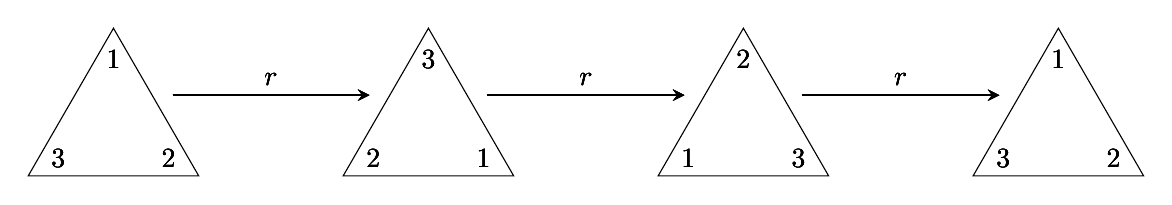
\begin{tikzpicture}[>=stealth]
\foreach \a in {1,2,3,4}{
	
	\node[regular polygon, regular polygon sides=3, minimum size=2.5cm, draw] at (\a*4-2.5,0) {};
	\node (v1) at (1.5,.85) {1};
	\node (v2) at (.8,-.4) {3};
	\node (v3) at (2.2,-.4) {2};
	\node (v4) at (5.5,.85) {3};
	\node (v5) at (4.8,-.4) {2};
	\node (v3) at (6.2,-.4) {1};
	\node (v6) at (9.5,.85) {2};
	\node (v7) at (8.8,-.4) {1};
	\node (v8) at (10.2,-.4) {3};
	\node (v9) at (13.5,.85) {1};
	\node (v10) at (12.8,-.4) {3};
	\node (v11) at (14.2,-.4) {2};
	
	\node (v12) at (3.5,.6) {$ r $};
	\node (v13) at (7.5,.6) {$ r $};
	\node (v14) at (11.5,.6) {$ r $};
	
	\draw[->,thick] (2.25,.4) -- (4.75,.4);
	\draw[->,thick] (6.25,.4) -- (8.75,.4);
	\draw[->,thick] (10.25,.4) -- (12.75,.4);
}
\end{tikzpicture}
Applying $ r $ a third time will bring us back to our starting position, or $ r^3=1 $. $ H=\{1,r,r^2\} $ is a nice subgroup.\\

Now do a flip,$ f $, about the altitude holding vertex $ 1 $ fixed. This looks like:

\begin{tikzpicture}[>=stealth]
\hspace{.25in}
\foreach \a in {1,2}{
	
	\node[regular polygon, regular polygon sides=3, minimum size=2.5cm, draw] at (\a*4+1.5,0) {};
	\node (v1) at (1.5,.85) {};
	\node (v2) at (.8,-.4) {};
	\node (v3) at (2.2,-.4) {};
	\node (v4) at (5.5,.85) {1};
	\node (v5) at (4.8,-.4) {3};
	\node (v3) at (6.2,-.4) {2};
	\node (v6) at (9.5,.85) {1};
	\node (v7) at (8.8,-.4) {2};
	\node (v8) at (10.2,-.4) {3};
	\node (v9) at (13.5,.85) {};
	\node (v10) at (12.8,-.4) {};
	\node (v11) at (14.2,-.4) {};
	
	\node (v12) at (3.5,.6) {};
	\node (v13) at (7.5,.65) {$ f $};
	\node (v14) at (11.5,.6) {};
	

	\draw[->,thick] (6.25,.4) -- (8.75,.4);

}
\end{tikzpicture}

The reader should check that $ r^2f $ ($ r^2 $ followed by $ f $, in that order) will yield another flip, one that pivots about vertex 3. The last symmetry, another flip, is given by $ rf $ which is a pivot about vertex 2.\clearpage
Summary: The six symmetries of an equilateral triangle can be expressed in terms of just $ r $ and $ f $. They are, $ \{1,r,r^2,f,rf,r^2f\} $.\\
In the problems you are asked to make the $ 6\times 6 $ operation table for these six symmetries. As you try to complete the table you may run into trouble with a few like $ fr, fr^2, frf $\dots\\

\begin{tcexample}{}{}
In the problems you are asked to draw a sequence of triangles to show $ fr=r^2f. $
\end{tcexample}

\begin{tcexample}{}{}
	$ fr^2=(fr)r=(r^2f)r=r^2r^2f=rf $
\end{tcexample}

\begin{tcexample}{}{}
$ frf=(fr)f=r^2ff=r^2 $.
\end{tcexample}

There is something convenient about switching to cycle notation. Notice that $ r=(132) $ and $ f=(23) $. It is not hard to see that $ r^2=(123) $ and $ rf=(13) $, $ r^2f=(12) $. Now we can be independent of the pictures, and generalizations are easier to see.\\
BIG CAUTION! Rotate the pictures clockwise, but perform composition of functions (cycles) \underline{right} to \underline{left} just as you do when computing $ f(g(x)) $. Now cycle form corresponds with the $ r-f $ version. 
\clearpage
\subsection{The Rectangle Group\\ (or how does the post office cancel stamps?)}\index{rectangle group}
There are four rigid motion symmetries of a rectangle.\\
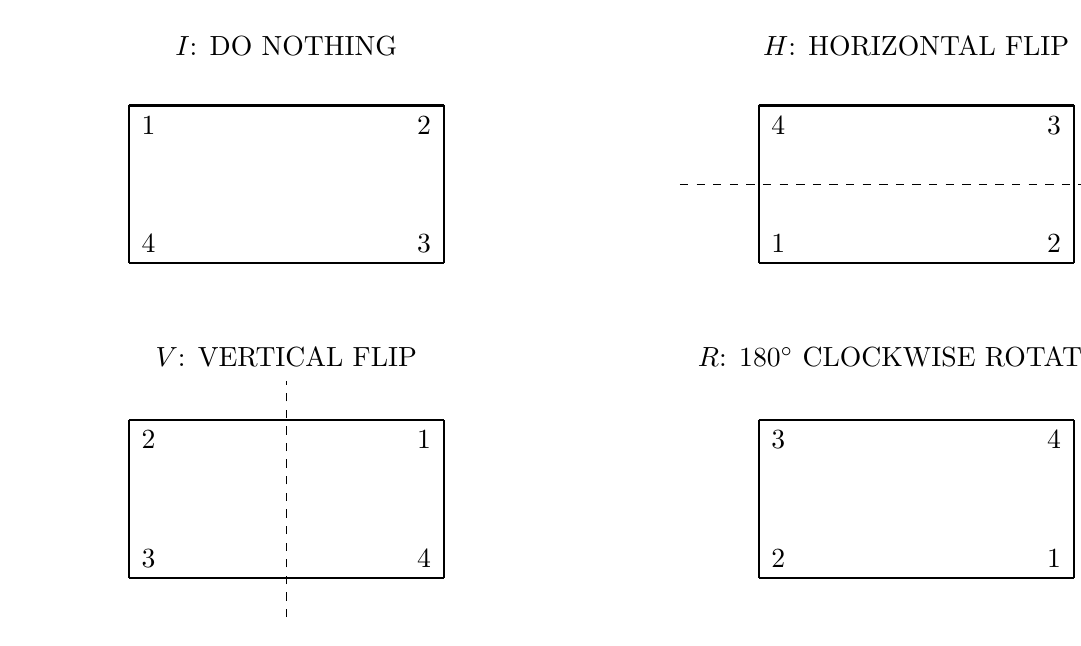
\begin{tikzpicture}{
\hspace{.5in}
\draw[-,thick](0,0) -- (0,2);
\draw[-,thick](0,0) -- (4,0);
\draw[-,thick](4,0) -- (4,2);
\draw[-,thick](0,2) -- (4,2);

\draw[-,thick](8,0) -- (8,2);
\draw[-,thick](8,0) -- (12,0);
\draw[-,thick](12,0) -- (12,2);
\draw[-,thick](8,2) -- (12,2);

\draw[dashed](7,1) -- (13,1);

\draw[-,thick](0,-4) -- (0,-2);
\draw[-,thick](0,-4) -- (4,-4);
\draw[-,thick](4,-4) -- (4,-2);
\draw[-,thick](0,-2) -- (4,-2);

\draw[dashed](2,-4.5) -- (2,-1.5);

\draw[-,thick](8,-4) -- (8,-2);
\draw[-,thick](8,-4) -- (12,-4);
\draw[-,thick](12,-4) -- (12,-2);
\draw[-,thick](8,-2) -- (12,-2);

\node (v1) at (.25,1.75) {1};
\node (v2) at (3.75,1.75) {2};
\node (v3) at (3.75,.25) {3};
\node (v4) at (.25,.25) {4};

\node (v5) at (8.25,1.75) {4};
\node (v3) at (11.75,1.75) {3};
\node (v6) at (11.75,.25) {2};
\node (v7) at (8.25,.25) {1};

\node (v8) at (.25,-2.25) {2};
\node (v9) at (3.75,-2.25) {1};
\node (v10) at (3.75,-3.75) {4};
\node (v11) at (.25,-3.75) {3};

\node (v12) at (8.25,-2.25) {3};
\node (v13) at (11.75,-2.25) {4};
\node (v14) at (11.75,-3.75) {1};
\node (v15) at (8.25,-3.75) {2};

\node (v16) at (10,2.75) {$H$: HORIZONTAL FLIP};
\node (v17) at (2,-1.2) {$V$: VERTICAL FLIP};
\node (v17) at (10,-1.2) {$R$: $180\degree$ CLOCKWISE ROTATION};

\node (v18) at (2,2.75) {$I$: DO NOTHING};
	
}
\end{tikzpicture}\\
The interior numbers indicate their movement from $ I $, the original position. The group table for $ G=\{I,H,V,R\} $ is shown next:
 \[
\begin{tabular}{>{$}l<{$}|*{4}{>{$}l<{$}}}
\circ   & ~I~  & ~H~   & ~V~ & ~R~      \\
\hline\vrule height 12pt width 0pt
~I   & ~I   & H  & V & R      \\
H   & H   & ~I   & R   & V      \\
V   & V   & R   & ~I   & H        \\
R   & R  & V  & H & ~I      \\

\end{tabular} 
\] 
$ G $ is evidently a Klein 4-group; the orders of $ H,V, \text{ and }R $ are 2.
\subsubsection{The Rectangle Group in Cycle Form}
It is easy to see that the following correspondence holds: $ I=(1), H=(14)(23), V=(12)(34) $ and $ R=(13)(24) $. In the problems you are asked to make the operation table for the rectangle group in cycle form.\\[.2in]
\underline{PROBLEMS - GROUPS OF SYMMETRIES}

\begin{enumerate}
	\item Draw a sequence of triangles to show that $ fr=r^2f $.
	\item Why is $ f^2=(1) $, the identity?
	\item Show that $ f(r^2f)=r $.
	\item Show that $ (r^2f)(rf)=r $.
	\item Make the multiplication table for $ \{1,r,r^2,f,rf,r^2f\} $.
	\item Make the multiplication table for $ \{(1),(132),(123),(23),(13),(12)\} $.
	\item Make the operation table for the rectangle group in cycle form.
	
\end{enumerate}
\clearpage
\fbox{ Activity 11 } - THE OCTIC GROUP \\[.2in]
The octic group\index{octic group} consists of the symmetries of a square: some rotations and flips about the diagonals and horizontal/vertical flips.  Start with
~\\
\begin{figure}[h!]
	\centering
	\begin{tikzpicture}
	\draw(6,0)--(6,3);
	\draw(6,0)--(9,0);
	\draw(9,0)--(9,3);
	\draw(6,3)--(9,3);
	
	
	
	
	
	
	
	\node (A) at (6.2, 2.7) {1};
	\node (B) at (8.8, 2.7) {2};
	\node (C) at (8.8, .3) {3};
	\node (D) at (6.2, .3) {4};
	
	
	
	\end{tikzpicture}
	
\end{figure}
~\\	
and let $ r $ be a $ 90^\circ $ clockwise rotation, and let $ f $ denote a flip about the diagonal fixing 1 and 3. Determine that there are 8 symmetries. The easiest are $ e,r,r^2,r^3.  $ Show that $ fr=r^3f $ and use this to complete the $ 8\times 8 $ operation table for the octic group $\{ e,r,r^2,r^3,f,rf,r^2f,r^3f\}. $\clearpage

\fbox{ Activity 12 } - A TETRAHEDRON \\[.2in] \index{tetrahedron}
List the 12 symmetries of a regular tetrahedron in cycle form. For example, spinning about vertex 1 gives two : (234) and (243). What is the other type? 

~\\
~\\
\begin{figure}[h!]
	\centering
	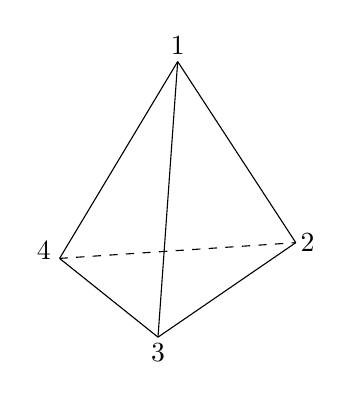
\begin{tikzpicture}
	\draw[dashed](6,0)--(9,.2);
	\draw(6,0)--(7.5,2.5);
	\draw(9,0.2)--(7.5,2.5);
	\draw(7.25,-1)--(7.5,2.5);
	\draw(7.25,-1)--(6,0);
	\draw(7.25,-1)--(9,.2);
	
	
	
	\node (A) at (7.5,2.7) {1};
	\node (B) at (9.15,.2) {2};
	\node (C) at (7.25, -1.2) {3};
	\node (D) at (5.8, .1) {4};
	
	
	
	
	
	
	
	
	\end{tikzpicture}
	
\end{figure}

\section{Quotient Groups}
\stepcounter{section}

\subsection{Cosets and Normal Subgroups}

Lagrange's Theorem states that the order of any subgroup $H$ divides the order of a (finite) group $G$. This is (was) proved by partitioning the elements of $G$
into nonoverlaping sets called \underline {cosets}.\index{coset} For $a\in G$ a (left) coset of $H$ is the set $\{aH\}$ consisting of all products $ah$ with $h\in H$. The number of cosets is called the \underline{index} of $H$ in $G$. A right coset is the set $\{Ha: a\in G\}$. If $aH = Ha$ for every $a\in G$, as sets, we say that $H$ is a \underline{normal} subgroup.\index{normal subgroup}  For an additive group, the notation $a+H = H+a$ is used.

\begin{tcexample}{}{}
Let $S_3 =\{1, r, r^2, f, rf, r^2f\}$ be the rigid transformations of an equilateral triangle. $H = \{1, f\}$ is not a normal subgroup: $rH = \{r, rf\}$, but $Hr = \{r, fr\}$ = $\{r, r^2f\}$. As sets, $rH \neq Hr$.
\end{tcexample}

\begin{tcexample}{}{}
	$H = \{1, r, r^2\}$   is a normal subgroup of $G=S_3$. $aH = Ha$ if $a\in H$. So now try the other three: $fH = \{f, r^2f, rf\}$ = $Hf$, $rfH = \{rf, f, r^2f\} = Hrf$, and also $r^2fH = Hr^2f$. So $aH = Ha$, for all $a\in G$.
\end{tcexample}

The good news is that if $G$ is abelian, all subgroups are normal. Here is another helpful result: If the index\index{index of a subgroup} of $H$ in $G$ is $2$, $H$ is normal. That's why it is easy to see that the $H$ in example $2$ is normal.

It turns out that if $H$ is normal you can multiply cosets! You get the following nice process: $aHbH = abH$. This is not hard to show: $abH\subseteq aHbH$ is easy to show. For $aHbH\subseteq abH$, use normality.

\begin{tctheorem}{}{}
Let $N$ be a normal subgroup of $G$. The product  $aNbN$ of cosets is the coset $abN$.
\end{tctheorem}

\begin{tctheorem}{}{}
 The (left) cosets of a normal subgroup $H$ in $G$ form a group.
\end{tctheorem}

\begin{newproof}
	\begin{enumerate}
	\item
	
	Closure: $aHbH$ = $abH$
	\item
	
	Identity: If $e$ is the identity in $G$, $eH$ is the identity in the new group since $eHaH$ = $eaH$ = $aH$ = $H$ = $aeH$ = $aH eH$.
	\item
	
	Inverses: The inverse of $aH$ is $a^{-1}H$ since $aHa^{-1}H$ = $a^{-1}aH$ = $H$ = $a^{-1}HaH$.
	\item
	
	Associativity: $aH(bHcH)$ = $aHbcH$ = $abcH$, and ($aHbH)cH$ = $abHcH$ = $abcH$.
\end{enumerate}

\end{newproof}


~\\
\underline{Definition.} If $N$ is a normal subgroup of $G$, the set of all left cosets $aN$ form a group called the \underline{QUOTIENT GROUP},\index{quotient group} or Factor Group,\index{factor group} denoted $G/N$.\\[.2in]

\begin{tcexample}{}{}
 Let $G$ = $\Z_6$ and $H$ = $\{0,3\}$. Since $\Z_6$ is abelian, $H$ is a normal subgroup. The three cosets are $H$, $1+H$ = $\{1,4\}$ and $2+H$ = $\{2,5\}$ and $G/H$ = $\{H, 1+H, 2+H\}$.
We next make the addition table for $\Z_6$, with the elements rearranged as $0, 3, 1, 4, 2, 5$; next to it  make the operation table for $G/H$:



\begin{center}
	\begin{tabular}{c||cc|cc|cc}
		$\oplus$ & 0 & 3 & 1 & 4 & 2 & 5 \\ \hline\hline
		0 & 0 & 3 & 1 & 4 & 2 & 5 \\
		3 & 3 & 0 & 4 & 1 & 5 & 2 \\ \hline
		1 & 1 & 4 & 2 & 5 & 3 & 0 \\
		4 & 4 & 1 & 5 & 2 & 0 & 3 \\ \hline
		2 & 2 & 5 & 3 & 0 & 4 & 1 \\
		5 & 5 & 2 & 0 & 3 & 1 & 4
	\end{tabular}
	\qquad\qquad
	\begin{tabular}{c | c c c}
		& $H$ & $1+H$ & $2+H$ \\ \hline
		$H$ & $H$ & $1+H$ & $2+H$ \\
		$1+H$ & $1+H$ & $2+H$ & $H$ \\
		$2+H$ & $2+H$ & $H$ & $1+H$
	\end{tabular}
\end{center}
~\\[.1in]

These two tables look almost the same!

There are several features of this example to notice:
\begin{enumerate}
	
	\item
	The three cosets partition the elements of $\Z_6$ into three disjoint sets.
	\item
	$H$ = $\{0,3\}$ is the identity coset.
	
	\item
	Some funny addition is going on: $(1+H)$ + $(2+H)$ = $\{1,4\}$ + $\{2,5\}$ = $\{1+2,1+5,4+2,4+5\}$ = $\{3,6,6,9\}$ = $\{0,3\}$ =$H$.
	
	\item
	The inverse of $1+H$ is $2+H$.
	\item
	The index of $H$ in $G$ is $3$.
\end{enumerate}
\end{tcexample}

\begin{tcexample}{}{}
 Let $G$ = $V_{15}$ = $\{1,2,4,7,8,11,13,14\}$ and $H$ =  $\{1,11\}$. $H$ is normal in $G$ (why?). The four cosets of $H$ are $H$, $2H$ = $\{2,7\}$,  $4H$ = $\{4,14\}$, and  $8H$ =   $\{8,13\}$. The quotient group table is:


\begin{center}
	\begin{tabular}{c|cccc}
		& $H$ & $2H$ & $4H$ & $8H$  \\ \hline
		$H$  & $H$ & $2H$ & $4H$ & $8H$  \\
		$2H$ & $2H$ & $4H$ & $8H$ & $H$  \\
		$4H$ & $4H$ & $8H$ & $H$ & $2H$  \\
		$8H$ & $8H$ & $H$ & $2H$ & $4H$
	\end{tabular}
\end{center}

~\\[.2in]
Which group of order 4 is this? $\Z_4$ or the Klein $4$-group?

\end{tcexample}

\begin{tcexample}{}{}
Let $G$ = $\Z$, and $H$ = $3\Z$. Then the cosets in $G/H$ are $0+H$, $1+H$ and $2+H$. If $H$ = $2\Z$ the cosets are simply the set of even integers, and the set of odd integers.
\end{tcexample}	
~\\[.2in]
\underline{PROBLEMS - QUOTIENT GROUPS}

\begin{enumerate}
	\item
	List the left cosets of the subgroup $3\Z$ in $\Z$. Now list the right cosets. These are the same since the additive group $\Z$ is an abelian group.
	
	\item
	List the left cosets of $H =\{1,rf\}$ in $S_3$. Now list the right cosets. What do you notice?
	\item
	Let $H = \{...,-10, -5,0,5,10,...\}$. Find all the left cosets of $H$ in $\Z$. Are $-3 + H$ and $-8+H$ in the same coset? Where would you find $21$? How about $-17$?
	\item
	Let $H = \{1,8\}$ be a subgroup of $V_9 =\{1,2,4,5,7,8\}$, the multiplicative group of the invertibles mod $9$. Make all left cosets of $H$ in $V_9$, and make the group table for $V_9/H$.
	\item
	$H=\{1,r,r^2\}$ is a normal subgroup of $S_3 =\{1,r,r^2,f,rf,r^2f\}$. Make the group table for the quotient group $S_3/H$.
	\item
	What is the size of $3 + H$ where $H=\{0,6,12\}$ is a subgroup of $\Z_{18}$? What is the order of $3 + H$ in $\Z_{18}/H$? Is this quotient group cyclic?
	\item
	If $G$ is an abelian group, explain why every subgroup of $G$ is normal.
	\item
	Determine the elements of the quotient group  for each of the following:
	\begin{enumerate}
		\item
		$G = \Z_{12}$~~    $H = \{0,4,8\}$
		\item
		$G = \Z$~~~~~            $H = 2\Z$
		\item
		$G = D_4$~         $H = \{1,r,r^2,r^3\}$ where $ D_4 $ is the group formed from the symmetries of a square
		\item
		$G = V_{15}$~~       $H = \{1,4,11,14\}$
		\item
		$G = V_{15}$~         $H = \{1,4\}$
	\end{enumerate}
	\item
	Let $G = [a]$ be a cyclic group of order $21$ generated by $a$, and let $H$ be a subgroup having index $3$.  List the elements of $H$ and the elements of $G/H$. Make the operation table for the quotient group $G/H$.
	\item
	Let $G$ be a cyclic group of order $91$ and $H$ be a subgroup having index $7$. List the cosets of the quotient group $G/H$.
	\item
	If the index of a subgroup $H$ in $G$ is $2$, prove that $H$ is normal.
	\item
	The six roots of $x^6-1 = 0$ form a multiplicative group $G = \{ 1,r,s,-1,-r,-s\}$ where 1, r, s are roots of $x^3-1=0$. Form the left cosets of $H =\{1,r,s\}$ and make the operation table for $G/H$.
	\item
	Let $G = \{000,001,010,011,100,101,110,111\}$ under bitwise addition mod $2$, and $H= \{000,011\}$. List the left cosets of $H$.
	\item
	The elements of the Quaternion group $G$ are $\{1,-1,i,-i,j,-j,k,-k\}$.\index{quaternion group} Find a normal subgroup $H$ and make the operation table for $G/H$.
	\item
	Prove that if $G$ is an abelian group, so is the quotient group $G/H$ for any normal subgroup $H$.
	\item
	Let $G=\Z_4\times \Z_4$ and let $N$ be the cyclic subgroup generated by the element $(3,2)$. Show that $G/N$ is isomorphic to $\Z_4$.
	\item
	$\mathbb{Q}/\Z$ is an additive abelian group, with infinite order. What is the order of the coset $2/7 + \Z$?
	\item
	$H = \{(x,5x): x\in \mathbb{R}\}$ is a subgroup of the additive group $\mathbb{R}\times \mathbb{R}$. Give a geometrical description of $H$ and of the coset $(2,7) + H$. What do the cosets of $H$ look like? What do the cosets of the circle group in the complex numbers look like?
	\item
	Let $N = \{(x,y):y = -x\}$ be a subgroup of the additive group $\mathbb{R}\times \mathbb{R}$. Describe the cosets of $N$.
\end{enumerate}
\section{A Brief Look at Rings}
\stepcounter{section}

This type of structure should ring a bell.  As in the integers $\Z$, in a ring we can add, subtract, multiply and even distribute.  So think of $\Z$ as our model of a ring.\\
\underline{Definition.} A \underline{ring} $R$ \index{ring} is a set with two binary operations such that
\begin{description}
\item[\quad(a)]$R$ is an abelian group under addition.
\item[\quad(b)]$R$ is closed and associative under multiplication.
\item[\quad(c)]Multiplication is distributive over addition, ie, $a(b+c)=ab+ac$ and $(b+c)a=ba+ca$.
\end{description}
A \underline{commutative ring} is a ring where $ab=ba$.\\
\begin{tcexample}{}{}
 $\Z,\mathbb{Q},\mathbb{R}, \text{ and } \mathbb{C}$ are commutative rings.
\end{tcexample}

\begin{tcexample}{}{}
$\Z_m$, the ring of integers modulo $m$, is commutative.
\end{tcexample}

\begin{tcexample}{}{}
The set $\Z[x]$ of all polynomials in $x$ with coefficients in $\Z$ is a commutative ring.
\end{tcexample}
~\\
\underline{Definition.} If a ring $R$ has a multiplicative identity $1$, then an element $a$ in $R$ is an \underline{invertible}\index{invertible} if there is an $a^{-1}$ such that $a\,a^{-1}=1$; $1$ is called the \underline{unity}.\index{unity of a ring}\\

\begin{tcexample}{}{}
 $2\Z$ is a commutative ring with no unity.
\end{tcexample}

\begin{tcexample}{}{}
$ (\Z,\oplus,\otimes) $ is a ring where $ a\oplus b=a+b-1 $ and $ a\otimes b= a+b-ab $. Closure under $ \oplus $ is clear since $ a\oplus b= a+b-1\in \Z $. The additive identity is 1 since $ a\oplus 1 = a+1-1=a=1\oplus a$. The inverse of $ a $ is $ 2-a $ since $ a\oplus (2-a)=a+2-a-1=1. $ The binary operation $ \oplus $ is associative since:\\
$ a\oplus(b\oplus c)=a\oplus (b+c-1)=a+b+c-2 $ and $ (a\oplus b)\oplus c= (a+b-1)\oplus c= a+b-1+c-1=a+b+c-2. $\\
Closure under multiplication is clear since $ a \otimes b= a+b-ab\in \Z $. Finally, we check distributivity: $ a\otimes (b \oplus c)= a \otimes (b+c-1)= a+b+c-1-(ab+ac-a) $ and $ ( a \otimes b)\oplus (a \otimes c)= (a+b-ab)\oplus (a+c-ac)= 2a+b+c-ab-ac-1. $ The reader should check that $ \otimes $ is associative.
\end{tcexample}
~\\
A \underline{subring} (like a subgroup)\index{subring} of a ring $R$ is a subset of $R$ that is a ring.  The set $\{0,\pm5,\pm10,\dots\}$ is a subring of $\Z$.\\[.2in]
\underline{PROBLEMS - A BRIEF LOOK AT RINGS}
\begin{enumerate}
\item Show that $\Z[\sqrt2]=\{a+b\sqrt2:a,b\in \Z\} $is a ring.
\item In a ring $R$, show that $a^2-b^2=(a+b)(a-b)$ if and only if $R$ is commutative.
\item Show that $\Z[i]=\{a+bi: a,b \in \Z\}$ is  a ring.  $\Z[i]$ is called the ring of \underline{Gaussian Integers}.\index{Gaussian integers}
\item Find all invertibles in $\Z[i]$.
\item Find the unity in $S=\{0,2,4,6,8\}$ under addition mod 10.
\item What are the invertibles in $\Z\times \Z$?
\item Let $R=\{0,1,c\}$ be a ring with unity.
\begin{enumerate}
\item Show that $1+1=c$ and that $1+1+1=0$.
\item Show that $c^2=1$.
\item Make the $\times$ and $+$ tables for $R$.
\end{enumerate}
\item Let $R=\{0,1,c,d\}$ be a ring (with unity 1) with $c,d$ invertibles.  Make the multiplication table for $R$.
\item For $ a,b\in \mathbb{Q} $, define $ \oplus $ and $ \otimes $ by $ a\oplus b=ab $ and $a \otimes b =a+b$. Is $ (\mathbb{Q},\oplus,\otimes) $ a ring?
\end{enumerate}

 \fbox{ Activity 13 } - COMPLETE THE RING \\[.2in]
Complete the multiplication table for the ring $ R=\{a,b,c,d\} $

\begin{multicols}{2}
	
	\[
	\begin{tabular}{>{$}l<{$}|*{4}{>{$}l<{$}}}
	+   & a  & b   & c & d      \\
	\hline\vrule height 12pt width 0pt
	a   & a   & b  & c & d      \\
	b   & b   & a   & d   & c      \\
	c   & c   & d   & a   & b        \\
	d   & d  & c  & b & a      \\
	
	\end{tabular} 
	\]
	
	\columnbreak 
	
	\[
	\begin{tabular}{>{$}l<{$}|*{4}{>{$}l<{$}}}
	*   & a  & b   & c & d      \\
	\hline\vrule height 12pt width 0pt
	a   & a   & a  & a  & a      \\
	b   & a   & b  & ~   &       \\
	c   & a  & ~   & ~   & a        \\
	d   & a   & b   & c  & ~      \\
	
	\end{tabular} 
	\]
	
\end{multicols}

\section{Integral Domains}
\stepcounter{section}

When you were asked to solve $x^2-7x+12=0$, you set each factor in $(x-3)(x-4)$ to zero and solved $x-3=0$ or $x-4=0$.  Now try that in $\Z_{12}$; you get 3, 4 and 7 as solutions.  This quadratic has three roots.\\
\underline{Definition.} If $a$ and $b$ are nonzero elements of a ring and $ab=0$, we call $a$ and $b$ \underline{0-divisors}.\\
\begin{tcexample}{}{}
n $\Z_{12}$, the 0-divisors are 2, 3, 4, 6, 8, 9, 10 since $2\cdot6=3\cdot4=8\cdot9=6\cdot10=0$ in $\Z_{12}$.  These seven elements are precisely those numbers not relatively prime to 12.
\end{tcexample}
~\\[.1in]
%
\underline{Definition.} An \underline{integral domain}\index{integral domain} is a commutative ring $D$ with a unity, that has no 0-divisors.
$$\begin{array}{c|c}
\text{These are} & \text{These are not}\\
\hline
\Z,\mathbb{Q},\mathbb{R} & \Z_6, \Z_{12}\\
\Z_p, p \text{ a prime} & \Z_m, m\text{ composite}\\
\Z[\sqrt2] & \Z\times \Z\\
\Z[x] & 2\Z\\
\Z[i] &  \Z_5[i]
\end{array}$$\\[.2in]

\newpage
\underline{PROBLEMS - INTEGRAL DOMAINS}
\begin{enumerate}
\item List all 0-divisors in $\Z_{20}$.  What are the invertibles?
\item Find all solutions to $x^2-4x+3=0$
\begin{enumerate}
\item in $\Z_{12}$
\item in $\Z_{11}$
\end{enumerate}
\item Find a 0-divisor in $\Z_5[i]=\{a+bi:a,b\in \Z_5\}$.
\item Show that $\Z\times \Z$, with multiplication and addition defined coordinatewise, is not an integral domain.
\item Why is $2\Z$ not an integral domain?
\item Let $S=\{a,b,c\}$ and $P(S)$ be the power set \index{power set $ P(S) $} of $S$, ie, the set of all subsets of $S$ including $\phi$ and $S$.  Define the product $AB$ to be $A\cap B$ and the sum $A+B$ to be $(A\cup B)-(A\cap B)$, the elements in $A\cup B$ but not those in $A\cap B$.
\begin{enumerate}
\item Show that $P(S)$ is a commutative ring.
\item What is the unity?
\item What acts like a ``0''?
\item Is $P(S)$ an integral domain?
\end{enumerate}
\item In $Z_6$ show that $ab=ac$ does \underline{not} imply $b=c$.
\item Show that $ M_2(\Z_2) $, the set of all $ 2\times 2 $ matrices with entries in $ \Z_2 $ with the usual matrix operations is not an integral domain.
\item Prove that right and left cancellation laws hold in a ring $ R $ if and only if $ R $ has no zero divisors. In other words, if $ c\neq 0 $ and $ c $ is not a $ 0 $-divisor, then either $ ac=bc $ or $ ca=cb $ implies $ a=b $.
\item Is the ring of Gaussian integers an integral domain?
\item Is the direct product of integral domains an integral domain?
\item Suppose $ D=\{0,d_2,d_3,\text{\dots},d_n\} $ is an integral domain. Prove that $\{d_2,d_3,\text{\dots},d_n\}$ is a multiplicative group. 
\end{enumerate}


\section{Fields -- The Finale}
\stepcounter{section}

A \underline{field}\index{field} is a commutative ring with unity where every nonzero element is an invertible.  In other words, a field is an integral domain whose nonzero elements form a multiplicative group.  More formally, a field $F$
\begin{description}
\item[\quad(a)] is an abelian group under addition
\item[\quad(b)] is an abelian group under multiplication (don't count 0)
\item[\quad(c)] has the property that multiplication is distributive over addition.
\end{description}

\begin{tcexample}{}{}
$\mathbb{Q},\,\mathbb{R},\,\mathbb{C},\,\Z_p,\, \mathbb{Q}[\sqrt2]$ are fields.
\end{tcexample}

\begin{tcexample}{}{}
$\Z_3[i],\, \Z_7[i]$ and $\Z_{11}[i]$ are fields; but $\Z_2[i],\, \Z_5[i]$ and $\Z_{13}[i]$ are not. [Note that when $p\equiv3(\text{mod }4),\, \Z_p[i]$ is a field].
\end{tcexample}

\begin{tctheorem}{}{}
 Every finite integral domain $D$ is a field.
\end{tctheorem}
\begin{newproof}
 Let $a\in D$ and $ a\neq0 $; we show that $a$ has a multiplicative inverse. Let $D=\{0,1,a_1,a_2, \dots, a_n\}$.  The elements $a{\cdot} 1, a\,a_1, a\,a_2, \dots, a\,a_n$ are surely distinct since $D$ is an integral domain, and none of these products is 0 since $D$ has no zero-divisors.\index{zero-divisor}  So one of these must be 1; let's say $a\,a_i=1$.  But then $a_i$ is the inverse of $a$.
\end{newproof}
\newpage
\underline{PROBLEMS - FIELDS}
\begin{enumerate}
\item Verify that $\mathbb{Q}[\sqrt2]$ is a field.  Show that $2+3\sqrt2$ has an inverse.
\item Why is $\Z_2[i]$ not a field?
\item Show that each of the following is not a field by finding 0-divisors:\\
(a) $ \Z_{13}[i] $. \qquad (b) $ \Z_{17}[i] $.
\item Is $\Z[\sqrt2]$ a field?
\item Let $F=\{0,2,4,6,8\}$ under addition and multiplication modulo 10.  Prove that $F$ is a field.
\item $ \Z_3[i] $ is a field with 9 elements.\\
(a) Make the 8 by 8 multiplication table.\\
(b) Make a table of inverses and orders of each element.\\
(c) Which familiar group is the multiplication group isomorphic to? 
\end{enumerate}
\vfill
\centerline{
\includegraphics[width=3in]{IMG_0454.JPG}}
\vfill


\section{Selected Answers}


~\\
%%%%% 1.BINARY OPERATIONS %%%%%

{\Large 1. \underline{Binary Operations}}

\begin{oddenumerate}
	\item \textbf{(a)} No; $ a-b \neq b-a $. \textbf{(b)} No. \textbf{(c)}Yes.
	\textbf{(d)} Yes; $ 1\cdot a=a$, No inverses. 
	
	\item \textbf{(a)} Yes; $ A\cup B= B\cup A $ \textbf{(b)} No; $\emptyset$ is the identity; no set in $ X $ satisfies $ \{a\}\cup X=\emptyset $.
	
	\item \textbf{(a)} $ 2\circ5 =175;~ 3\circ2=625 $ \textbf{(b)} No; no identity.
	
	\item Easy.
	
	\item $ e=10 $; no inverses.
	
	\item \textbf{(a)} Yes. \textbf{(b)} $ e=1 $ since $ 1 \square a= 1+a-1=a=a\square 1 $. \textbf{(c)} Yes; the inverse of $ m $ is $ 2-m $ since $ m\square(2-m)=2-1=1. $
	
	\item \textbf{(a)} No; $ 1\square 2=6 $, but $ 2\square 1=9 $. \textbf{(b)} Three, you should find these.
	
	\item Try $ 1\square 0 \square 2 $ and then $ 0 \square 1 $ for commutativity. 
	
	\item \textbf{(a)} No; $ 2^3\neq 3^2 $. \textbf{(b)}No, try $ 2\square1\square3 $. \textbf{(c)}$ a^{(b^c)}. $
	
	
\end{oddenumerate}


%%%%% 2.CLOSURE %%%%%
~\\[.1in]
{\Large 2. \underline{Closure}}

\begin{oddenumerate}
	\item \textbf{(a)} No; $ 1+4=5 $.  \textbf{(b)}No; $4-1=3.  $  \textbf{(c)} Yes, $ a^2b^2=(ab)^2 $
	
	\item  No; $ 4+6=10 \notin C $.
	
	\item  \textbf{(a)} No; $ 1+4=5 $,  \textbf{(b)} Yes; $ (3h+1)(3k+1)=9hk+3(h+k)+1. $
	
	\item $ H=\{0,\pm6,\pm12,\dots\} $; $ G\cap H=\{0,\pm12,\pm24,\dots\}, ~ 12h-12k=12(h-k). $
	
	\item Yes; yes.
	
	\item No
	
	\item Let $ S $ be closed under subtraction. If $ a\in S, a-a=0 \in S. $
	
	\item  \textbf{(a)} $ 5=1+4,~ 13=4+9, ~ 65=1+64 $. {\textbf{(b)} Yes, we can derive that \\$ (m_1^2+n_1^2)(m_2^2+n_2^2)= (m_1m_2-n_1n_2)^2+(n_1m_2+m_1n_2)^2$} 
	
	\item Yes
	
	\item 7 and 9
	
	
\end{oddenumerate}

%%%%% 3.GROUPS %%%%%
~\\[.1in]
{\Large 3. \underline{Groups}}

\begin{oddenumerate}
	\item Check the four axioms.
	
	\item The identity is $ 16. $
	
	\item $ 7^1=7,7^2=9, 7^3=3, 7^4=1; 9^1=9, 9^2=1 $
	
	\item $G$ is cyclic and generated by $ i $ or $ -i. $
	
	\item $ G=\{00,01,10,11\} $ under bitwise addition $\mod 2 $. 
	
	\item Mimic the table for $ B^2 $; $ G $ is Abelian, but not cyclic. 
	
	\item $ 0 $ is the additive identity; the inverse of $ 7a $ is $ -7a. $
	
	\item $ \{0\}, \{0,3\}, \{0,2,4\} $ and $ \mathbb{Z}_6 $ are the subgroups of $ \mathbb{Z}_6. $
	
	\item $ \{0\},\{0,6\}, \{0,3,6,9\}, \{0,4,8\}, \{0,2,4,6,8,10\},\text{ and } \mathbb{Z}_{12} $ are the subgroups of $\mathbb{Z}_{12}.  $
	
	\item The elements $ 0 $ and $ 2 $ have no inverses.
	
	\item $ 1,2,3,4 $ are generators. For example, $ 0\cdot 2=0,~ 1\cdot 2=2, 2+2=4,~ 2+2+2=1,~ 2+2+2+2=3. $
	
	\item \textbf{(a)} $ 0,3 $. \textbf{(b)} $ 0,4. $ \textbf{(c)} $ 0,2,3,5. $
	
	\item The identity is $ a^0=1 $; The inverse of $ a^h $ is $ a^{-h} $. Since $ a^ha^k=a^{h+k} $, $ H $ is closed. 
	
	\item The identity is $\begin{pmatrix} 0 & 0\\ 0 & 0 \end{pmatrix}$; the inverse of  $\begin{pmatrix} a & b\\ c & d \end{pmatrix}=  \begin{pmatrix} -a & -b\\ -c & -d \end{pmatrix}$.
	\item $ 0x+0 $ is the identity; the inverse of $ ax+b $ is $ -ax-b. $
	
	\item $ (ab)^{k+1}=(ab)(ab)^k=(ab)(a^kb^k)=(ba)(a^kb^k)=ba^{k+1}b^k=a^{k+1}b^{k+1} $ since $ b $ commutes with $ a $.
	
	
	
\end{oddenumerate}

%%%%% 4.MORE ON CYCLIC GROUPS %%%%%
~\\[.1in]
{\Large 4. \underline{More on Cyclic Groups}}

\begin{oddenumerate}
	\item  $ V_9 $ is cyclic with $ 2 $ as a generator. 
	
	\item $ H=\{e,a^8,a^{16}\} $; $ o(a^5)=24. $ List $ (a^5)^k $ for $ k=0,1,\dots, 24. $
	
	\item $\{1,3,7,9\}$ is cyclic. $ G=[3]. $
	
	\item $ 6 $; $ [25]=\{0,25,20,15,10,5\} $
	
	\item \textbf{(a)} 6. \textbf{(b)} 6. \textbf{(c)} 8. \textbf{(d)} 16.
	
	\item \textbf{(a)} $\omega$ is a root of $ \omega^3-1=(\omega-1)(\omega^2+\omega+1). $ \textbf{(b)} $\omega^3-1=0$. \textbf{(c)} 22. \textbf{(d)} 8, since $ (\cos\frac{\pi}{4}+i\sin\frac{\pi}{4})^8=1 $ and no lower power yields $ 1 $. \textbf{(e)} $ \infty $; start taking powers using De Moivre's Theorem.
	
	
	\item \textbf{(a)} 3. \textbf{(b)} 2. 
	
\end{oddenumerate}


%%%%% WILSON'S THEOREM %%%%%
~\\[.1in]
{\large ~~ \underline{Wilson's Theorem}}\index{Wilson's Theorem}

\begin{oddenumerate}
	\item  $ 2\cdot 7 \equiv 3\cdot 9 \equiv 4\cdot 10 \equiv 5\cdot 8 \equiv 6\cdot 1$ leaving $ 12\equiv -1(13) $.
	
	\item $ 2\cdot 3 \cdot 4\cdot \dots \cdot p-2 $ has an even number of elements $ x $ that pair up with $ x^{-1} $. Now use $ x\cdot x^{-1} $.
	
	\item Use $ (p-2)! \equiv 1(p). $
	
	\item[6.] $ x=1 $ or $ x=-1. $ If $ x^2-1=(x-1)(x+1)\equiv 0(p) $, then $ x=1  $ or $ x=-1 $. Since $ (x+1)-(x-1)=2 $, either $ p \vert (x+1) $ or $ p \vert (x-1) $, but not both. 
	
	\item Hints: $ 30 \equiv -29(59) $ and $ 31\equiv -30(61) $.
	
\end{oddenumerate}

%%%%% 5.LAGRANGE'S THEOREM %%%%%
~\\[.1in]
{\Large 5. \underline{Lagrange's Theorem}}

\begin{oddenumerate}
	\item  $ H=\{0,6\} $, $ 1+H=\{1,7\} $, $ 2+H=\{2,8\}, 3+H=\{3,9\}, 4+H=\{4,10\}, $ and $ 5+H=\{5,11\}. $ 
	
	\item $ V_9=\{1,2,4,5,7,8\}; H=\{1,8\}, 2H=\{2,7\}, 4H=\{4,5\}$. $ \{1,4,7\} $ is another subgroup. 
	
	\item If $ o(G)=p, $ then by Lagrange's Theorem every element $ g\neq e $ has order $ p $. So any one of these is a generator. 
	
	\item $ 1,3,5,9,15,45. $
	
	\item $ H=\{e,a^{13}, a^{26},\dots ,a^{78}\} $ has order 7; hence the index is 13. 
	
	
\end{oddenumerate}

%%%%% 6.ISOMORPHISMS %%%%%
~\\[.1in]
{\Large 6. \underline{Isomorphisms}}

\begin{oddenumerate}
	\item $\theta(x)=2x.$ 
	
	\item For onto, choose $ b\in \mathbb{R}^+ $, then solve $ 2^x=b  $ for $ x=\log_2b $. For one-to-one, if $ a\neq b \text{ in } \mathbb{R},  2^a \neq 2^b$ in $ \mathbb{R}^+. $
	
	\item Try $ \theta(x)=\ln x $.
	
	\item $ \theta(e)\theta(e)=\theta(ee)=\theta(e)=e'\theta(e). $ Right cancellation gives $ \theta(e)=e'. $ $ xx^{-1}=e $ gives $ \theta(x)\theta(x^{-1})=\theta(e)=e' $ and so $ \theta(x^{-1})=[\theta(x)]^{-1} $.
	
	\item Let $ \theta(a)=a' $ and let $ o(a)=q $ and $ o(a')=q' $, then $ e=a^q $ and $ \theta(a^q)=[\theta(a)]^{q} $. So $ [\theta(a)]^q=e'. $ Since $ q' $ is the least integer $ m $ with $ [\theta (a)]^m=e', $ we have $ q \geq q' $. Similarly, $ q'\geq q $ and hence $ q=q'. $
	
	\item Since $ \sqrt{xy}=\sqrt{x}\sqrt{y} $, $ \theta(xy)=\theta(x)\theta(y). $ $ \theta $ is one-to-one and onto. 
	
	\item $ V_{12}=\{1,5,7,11\}.~ \theta(1)=1, \theta(3)=5, \theta(5)=7, \theta(7)=11 $ is an isomorphism. Alternatively, they are both Klein 4-groups. 
	
	\item $ -1 $ has order $ 2 $ in $ (\mathbb{R}^*,\times) $, but $ (\mathbb{R}^+,\times) $ has no element of order $ 2 $, since $ x^2=1 \implies x=1 $.
	
	\item Let $ a\in \mathbb{Q} $ and suppose $\theta(a)=-1$; $-1$ must have a preimage if $\theta$ is an isomorphism. Then $-1=\theta (\frac{a}{2}+\frac{a}{2}) = [\theta(\frac{a}{2})]^2$, a contradiction. 
	
	
\end{oddenumerate}


%%%%% 7. DIRECT PRODUCTS %%%%%
~\\[.1in]
{\Large 7. \underline{Direct Products}}

\begin{oddenumerate}
	\item Yes; you should compute $ m(1,2) $ for $ m=0,1,\dots, 5. $
	
	\item No; Yes. $ (1,1) $ is a generator for $ \mathbb{Z}_3 \times \mathbb{Z}_4. $ In fact, $ \mathbb{Z}_3 \times \mathbb{Z}_4 $ is isomorphic to $ \mathbb{Z}_{12} $, a cyclic group. 
	
	\item $ 60; o(3) $ in $ \mathbb{Z}_4 $ is $ 4 $; $ o(10) $ in $ \mathbb{Z}_{12} $ is $ 6; o(9) $ in $ \mathbb{Z}_{15} $ is $ 5 $. LCM$ (4,6,5)=60. $
	
	\item No; compare orders
	
	\item \textbf{(a)} 1. \textbf{(b)} 1. \textbf{(c)} 1. \textbf{(d)} 1. \textbf{(e)} 1.
	
	\item $ \mathbb{Z}_{16},\mathbb{Z}_4 \times \mathbb{Z}_4, \mathbb{Z}_2 \times \mathbb{Z}_8, \mathbb{Z}_2 \times \mathbb{Z}_2\times \mathbb{Z}_4 , \mathbb{Z}_2 \times \mathbb{Z}_2 \times \mathbb{Z}_2 \times \mathbb{Z}_2 $. You should compare orders to see which one it is. 
	
	\item $ \mathbb{Z}_3 \times \mathbb{Z}_5$ is one possibility. How about $ [(2,0)] $ or $ [(10,4)] $. There are others. 
	
	\item $ o(9)=10; o(21)=10 $. $ 9 $ is the inverse of $ 21 $ since $ 9+21\equiv 0 $. In general, $ o(x)= o(x^{-1}) .$
	
	\item Let $ G_1 $ and $ G_2 $ be Abelian groups. Choose $(a,b) \text{ and } (c,d)\in G_1\times G_2.$ Then $(a,b)(c,d)=(ac,bd)=(ca,db)=(c,d)(a,b) $.
	
	
	
	
\end{oddenumerate}


%%%%% 8. PREMUTATION GROUPS %%%%%
~\\[.1in]
{\Large 8. \underline{Permutation Groups}}

\begin{oddenumerate}
	\item $ (13)(24) $
	
	\item $ (1 a b c d)= (1 a)(1 b)(1 c)(1 d) $ and similarly for an $ n- $cycle.
	
	\item $ (124)(356) $
	
	\item $ (142) $
	
	
	
	
	
	
\end{oddenumerate}


%%%%% 9. SYMMETRIES OF AN EQUILATERAL TRIANGLE %%%%%
~\\[.1in]
{\Large 9. \underline{Symmetries of an Equilateral Triangle}}

\begin{oddenumerate}
	\item[2.] A flip, followed by a flip, brings you back to the starting point.
	
	\item[3.] $ fr^2f=(fr)(rf)=r^2frf=r^2r^2ff=r^4f^2=r. $
	
\end{oddenumerate}	

%%%%% 10. QUOTIENT GROUPS %%%%%
~\\[.1in]
{\Large 10. \underline{Quotient Groups}}\index{quotient group}

\begin{oddenumerate}
	\item $ 3\mathbb{Z}, 1+3\mathbb{Z}, 2+3\mathbb{Z} ; 3\mathbb{Z}, 3\mathbb{Z}+1, 3\mathbb{Z}+2. $
	
	\item $ H, 1+H, 2+H, 3+H, 4+H; $ Yes; $ 21\in 1+H, -17\in 3+H. $
	
	\item $ H=\{1,r,r^2\} $ and $ fH=\{f,r^2f,rf\} $ are the only cosets.
	
	\item $ aH=Ha $ for all $ a\in G $ and every subgroup $ H $.
	
	\item $ H=\{e,a^3,a^6,a^9,a^{12},a^{15},a^{18}\}; G/H=\{H,aH,a^2H\} $
	
	\item If the index is 2, there are only two cosets, say $ H $ and $ aH $. But then $ Ha $ must be either $ H $ or $ aH $, so $ Ha=Ha $ since $ Ha\neq H. $
	
	\item $ 001+H=\{001,010\}, 100+H=\{100,111\}, 101+H=\{101,110\}. $
	
	\item $ aH\cdot bH=abH=baH=bHaH $
	
	\item Order of $\frac{2}{7}+\mathbb{Z}$ is $ 7 $ since $ 7(\frac{2}{7}+\mathbb{Z})=2+\mathbb{Z}=\mathbb{Z} $.
	
	\item Lines parallel to $ y=-x. $
	
\end{oddenumerate}


%%%%% INTEGRAL DOMAINS %%%%%
~\\[.1in]
{\large~~  \underline{Integral Domains}}

\begin{oddenumerate}
	\item  $ 2,4,5,6,8,10,12,14,15,16,18 $. The invertibles are $ 1,3,7,9,11,13,17,19. $
	
	\item $ (1+2i)(1+3i)= 1+5i-6=0; $ or $ (2+i)(2-i)=0. $
	
	\item No unity.
	
	\item $ 2\cdot 4= 2\cdot 1 $, but $ 4\neq 1. $
	
	\item If $ R $ has no $ 0- $divisors, then $ ac=bc $ implies $ ac-bc=(a-b)c=0 $ and so $ a-b=0 $ since $ c\neq 0. $ You should now prove the converse. 
	
	\item No. $ (0,1)(1,0)=(0,0) $.
	
\end{oddenumerate}


%%%%% 11. A BRIEF LOOK AT RINGS %%%%%
~\\[.1in]
{\Large 11. \underline{A Brief Look at Rings}}

\begin{oddenumerate}
	\item Check the three ring properties. For example, $ (a+b\sqrt{2})(c+d\sqrt{2})=ac+(bc+ad)\sqrt{2}+2bd $ shows closure under multiplication.
	
	\item Check Properties. $ (a+bi)(c+di)=ac-bd+(bc+ad)i $ shows closure under multiplication.
	
	\item 6 is the unity.
	
	\item \textbf{(a)} First make the addition table, then $ 1+1=c, 1+1+1=c+1=0 $. \textbf{(b) }$ c^2=(1+1)(1+1)=1+1+1+1=0+1=1. $
	
	\item Distributivity fails. $ 1 \otimes (2\oplus3)=1\otimes6=7 $. But $ (1\otimes 2)\oplus(1\otimes 3)=3\oplus4=12. $
	
	
	
	
\end{oddenumerate}

%%%%% 12. FIELDS %%%%%
~\\[.1in]
{\Large 12. \underline{Fields}}

\begin{oddenumerate}
	\item $ \frac{1}{2+3\sqrt{2}}= \frac{1}{2+3\sqrt{2}}\cdot\frac{2-3\sqrt{2}}{2-3\sqrt{2}}=\frac{2-3\sqrt{2}}{-14} =-\frac{1}{7}+\frac{3}{14}\sqrt{2}$
	
	\item \textbf{(a)} $ (2+3i)(2-3i)=4+9=0 $ \textbf{(b)}$ (4+i)(4-i)=0 $
	
	\item 6 is the unity; $ 2\cdot 8\equiv 4\cdot4 \equiv 6\cdot6\equiv 8\cdot 2 \equiv 6 $ provides inverses. 
	
	
	
	
\end{oddenumerate}
\backmatter

\printindex



\clearpage


\clearpage
\pagestyle{empty}

\cleardoublepage

% \thispagestyle{empty}
\begin{tikzpicture}[remember picture,overlay]
	\node[inner sep=0] at (current page.center){%
		\includegraphics[width=8in]{newworkbookcp.pdf}};
\end{tikzpicture}

\cleardoublepage
\phantomsection{}
\addcontentsline{toc}{section}{Workbook}
\includepdf[pages=2-]{workbook.pdf}

\cleardoublepage
\end{document}
